% ============================================================================
%  Frode-bibelen  --  PROG1001 Grunnleggende programmering (C), NTNU
%  Oppslagsverk til skoleeksamen (alle trykte og skrevne hjelpemidler).
%
%  HOVEDFIL. Kompiler denne med pdfLaTeX. Første gang trengs tre kjøringer før
%  innholdsfortegnelsen får riktige sidetall -- eller bruk latexmk:
%      latexmk -pdf frode-bibelen.tex
%  På Overleaf: last opp hele zip-filen som nytt prosjekt; hovedfilen velges
%  automatisk.
%
%  Struktur:
%      oppsett.tex          pakker, farger, kodestil, bokser, topptekst
%      forside.tex          forside og kolofon (hvit/mørk: se oppsett.tex)
%      kapitler/NN-*.tex    ett kapittel per fil, i to deler som følger eksamen:
%                           Del 1 (kapittel 2--8) = oppgave 1,
%                           Del 2 (kapittel 9--16) = oppgave 2
%
%  TIPS: Legg Frodes egen LesData.h i samme mappe som denne filen, så blir
%  den automatisk tatt med i kapittel 10.
%
%  Lisens: Beerware (Revision 42) -- se LICENSE.
% ============================================================================
\documentclass[10pt,a4paper]{article}
% !TEX root = frode-bibelen.tex
% ----------------------------------------------------------------------------
%  Frode-bibelen -- oppsett: pakker, farger, kodestil, bokser og topptekst
%  Inkluderes fra frode-bibelen.tex (kompiler alltid hovedfilen).
% ----------------------------------------------------------------------------

\usepackage[utf8]{inputenc}
\usepackage[T1]{fontenc}
\IfFileExists{norsk.ldf}
  {\usepackage[norsk,shorthands=off]{babel}}
  {\usepackage[english,shorthands=off]{babel}
   \addto\captionsenglish{\renewcommand{\contentsname}{Innhold}%
     \renewcommand{\figurename}{Figur}\renewcommand{\tablename}{Tabell}}}

\usepackage{charter}                       % brødtekst
\usepackage[scaled=0.92]{helvet}           % overskrifter
\renewcommand{\ttdefault}{txtt}            % kode
\usepackage{microtype}
\usepackage{pifont}

\usepackage[a4paper,margin=1.8cm,top=2.1cm,bottom=2.0cm,headsep=0.5cm]{geometry}
\usepackage[table]{xcolor}
\usepackage{listings}
\usepackage[skins,breakable]{tcolorbox}
\usepackage{fancyhdr}
\usepackage{titlesec}
\usepackage{enumitem}
\usepackage{booktabs}
\usepackage{array}
\usepackage{longtable}
\usepackage{multicol}
\usepackage{tikz}
\usetikzlibrary{positioning,arrows.meta,calc,shapes.multipart}
\usepackage[hidelinks]{hyperref}

% ---------------------------------------------------------------- farger ---
\definecolor{frodeblue}{HTML}{1F4E79}
\definecolor{kw}{HTML}{1F3F9F}
\definecolor{cm}{HTML}{4F7A4F}
\definecolor{st}{HTML}{9A2A2A}
\definecolor{bg}{HTML}{F5F7FA}
\definecolor{skinn}{HTML}{1C120E}          % mørkt skinn (forside)
\definecolor{skinnlys}{HTML}{3B271D}
\definecolor{gull}{HTML}{D4AF37}
\definecolor{gullmork}{HTML}{A88A2E}

% Forside: \morkforsidefalse = hvit bakgrunn med gullramme (for utskrift).
%          \morkforsidetrue  = svart skinn og gull (for skjerm/PDF).
\newif\ifmorkforside
\morkforsidefalse

% ------------------------------------------------------------- listings ---
\lstdefinestyle{frode}{
  language=C,
  basicstyle=\ttfamily\footnotesize,
  keywordstyle=\bfseries\color{kw},
  commentstyle=\color{cm},
  stringstyle=\color{st},
  morekeywords={bool,true,false,NULL,FILE},
  showstringspaces=false,
  columns=fullflexible, keepspaces=true,
  tabsize=2,
  breaklines=true,
  backgroundcolor=\color{bg},
  frame=leftline, framerule=2pt, rulecolor=\color{frodeblue!45},
  xleftmargin=8pt, framexleftmargin=5pt,
  aboveskip=6pt, belowskip=6pt,
  upquote=true,
  literate={æ}{{\ae}}1 {ø}{{\o}}1 {å}{{\aa}}1
           {Æ}{{\AE}}1 {Ø}{{\O}}1 {Å}{{\AA}}1
           {é}{{\'e}}1 {É}{{\'E}}1 {–}{{--}}1
           {«}{{\guillemotleft}}1 {»}{{\guillemotright}}1
}
\lstset{style=frode,basicstyle=\ttfamily\small}
\lstnewenvironment{kode}[1][]{\lstset{style=frode,#1}}{}
\newcommand{\cc}[1]{\texttt{#1}}            % kode i tabeller
\newcommand{\bs}{\textbackslash}

% ---------------------------------------------------------------- bokser ---
\tcbset{fbase/.style={enhanced,boxrule=0.6pt,arc=2pt,
  left=5pt,right=5pt,top=3pt,bottom=3pt,fonttitle=\sffamily\bfseries\small,
  before skip=6pt, after skip=6pt}}
\newtcolorbox{tips}[1][Tips]{fbase,colback=green!4,colframe=green!40!black,title={#1}}
\newtcolorbox{felle}[1][Felle]{fbase,colback=red!4,colframe=red!55!black,title={#1}}
\newtcolorbox{regel}[1][Regel]{fbase,colback=frodeblue!5,colframe=frodeblue,title={#1}}
\newtcolorbox{frode}[1][Frode sier]{fbase,colback=yellow!7,colframe=orange!70!black,title={#1}}

% ----------------------------------------------------------- overskrifter ---
\titleformat{\section}
  {\Large\sffamily\bfseries\color{frodeblue}}
  {\colorbox{frodeblue}{\color{white}\,\thesection\,}}{0.6em}{}
  [\vspace{-0.5em}{\color{frodeblue}\rule{\linewidth}{0.8pt}}]
\titleformat{\subsection}
  {\large\sffamily\bfseries\color{frodeblue!85!black}}{\thesubsection}{0.5em}{}
\titleformat{\subsubsection}
  {\normalsize\sffamily\bfseries}{\thesubsubsection}{0.5em}{}
\titlespacing*{\section}{0pt}{0pt}{10pt}
\titlespacing*{\subsection}{0pt}{12pt}{4pt}
\titlespacing*{\subsubsection}{0pt}{8pt}{2pt}
\newcommand{\kapittel}[1]{\clearpage\section{#1}}
% Bredere nummerfelt i innholdsfortegnelsen, så «12.10» ikke kolliderer med tittelen.
\makeatletter
\renewcommand*\l@subsection{\@dottedtocline{2}{1.5em}{2.8em}}
\makeatother

% Skilleside for Del 1 / Del 2 (egen side uten topptekst, med i innhold og bokmerker).
% Bruk: \del{Del 1 -- Oppgave 1}{Undertittel}
\newcommand{\del}[2]{%
  \clearpage\thispagestyle{empty}%
  \phantomsection\addcontentsline{toc}{part}{#1}%
  \vspace*{\fill}
  \begin{center}
    {\LARGE\sffamily\bfseries\color{frodeblue}#1\par}
    \vspace{8pt}\rule{0.45\linewidth}{0.6pt}\par\vspace{6pt}
    {\small #2\par}
  \end{center}
  \vspace*{\fill}\vspace*{3cm}
  \clearpage}

% Avkrysningsboks til sjekklistene (kapittel 1, 7 og 16).
\newcommand{\boks}{\raisebox{-0.2ex}{\setlength{\fboxsep}{0pt}\fbox{\rule{0pt}{1.5ex}\hspace{1.5ex}}}\ }

% ------------------------------------------------------------ topptekst ---
\pagestyle{fancy}
\fancyhf{}
\renewcommand{\sectionmark}[1]{\markboth{\thesection\quad #1}{}}
\fancyhead[L]{\sffamily\small\color{frodeblue}\textbf{Frode-bibelen}\ \textperiodcentered\ PROG1001}
\fancyhead[R]{\sffamily\small\leftmark}
\fancyfoot[C]{\sffamily\small\thepage}
\renewcommand{\headrulewidth}{0.4pt}

\setlist{nosep,leftmargin=1.4em}
\setlength{\parindent}{0pt}
\setlength{\parskip}{4pt}
\renewcommand{\arraystretch}{1.25}
\newcolumntype{L}[1]{>{\raggedright\arraybackslash}p{#1}}


% Vil du bare kompilere noen kapitler mens du jobber (raskere), fjern % under
% og list dem opp. Sidetall og kryssreferanser beholdes fra forrige fulle kjøring.
% \includeonly{kapitler/12-maler,kapitler/13-filer}

\begin{document}

% !TEX root = frode-bibelen.tex
% ----------------------------------------------------------------------------
%  Frode-bibelen -- forside og kolofon
%  Inkluderes fra frode-bibelen.tex (kompiler alltid hovedfilen).
% ----------------------------------------------------------------------------

% =============================================================== FORSIDE ===
\hypersetup{pageanchor=false}
\begin{titlepage}
\thispagestyle{empty}
\ifmorkforside
  \colorlet{omslag}{skinn}\colorlet{omslaglys}{skinnlys}
  \colorlet{forsidetekst}{gull}\colorlet{ramme}{gull}\colorlet{ramme2}{gullmork}
\else
  \colorlet{omslag}{white}\colorlet{omslaglys}{white}
  \colorlet{forsidetekst}{skinn}\colorlet{ramme}{gullmork}\colorlet{ramme2}{gull}
\fi
\newsavebox{\asciiboks}\newsavebox{\asciiskygge}
\begin{lrbox}{\asciiboks}\begin{minipage}{7.2cm}
\begin{lstlisting}[language={},backgroundcolor={},frame=none,xleftmargin=0pt,framexleftmargin=0pt,aboveskip=0pt,belowskip=0pt,columns=fixed,keepspaces=true,upquote=true,breaklines=false,literate={},basicstyle=\ttfamily\bfseries\fontsize{11.5}{12.4}\selectfont\color{forsidetekst}]
           cC
          cC
          cC
           cC
            cCc
              cC
               cC
                cC
                cC
                cC
c               cC
Cc     .-'\    cC
 Cc   /\   \  cC
  Cc. \ \   \cC  .-'\
   `Cc.\ \   \.-'    \
     `Cc\ \        .-/
        .-'     .-'.-'
     .-'        \-'
    /\    .-/\   \
    \ \.-'.-\ \   \
     \/.-'   \ \   \
              \ \   \
               \ \   \
                \ \   \
                 \ \   \
                  \ \   \
                   \ \   \
                    \ \_-/
                     \/-'
\end{lstlisting}
\end{minipage}\end{lrbox}
\begin{lrbox}{\asciiskygge}\begin{minipage}{7.2cm}
\begin{lstlisting}[language={},backgroundcolor={},frame=none,xleftmargin=0pt,framexleftmargin=0pt,aboveskip=0pt,belowskip=0pt,columns=fixed,keepspaces=true,upquote=true,breaklines=false,literate={},basicstyle=\ttfamily\bfseries\fontsize{11.5}{12.4}\selectfont\color{black}]
           cC
          cC
          cC
           cC
            cCc
              cC
               cC
                cC
                cC
                cC
c               cC
Cc     .-'\    cC
 Cc   /\   \  cC
  Cc. \ \   \cC  .-'\
   `Cc.\ \   \.-'    \
     `Cc\ \        .-/
        .-'     .-'.-'
     .-'        \-'
    /\    .-/\   \
    \ \.-'.-\ \   \
     \/.-'   \ \   \
              \ \   \
               \ \   \
                \ \   \
                 \ \   \
                  \ \   \
                   \ \   \
                    \ \_-/
                     \/-'
\end{lstlisting}
\end{minipage}\end{lrbox}
\begin{tikzpicture}[remember picture,overlay]
  % Skinnomslag med svak lysning på midten
  \shade[inner color=omslaglys, outer color=omslag]
        (current page.south west) rectangle (current page.north east);
  % Falsen ved ryggen (venstre kant)
  \ifmorkforside
    \fill[black,opacity=.35] ([xshift=0.95cm]current page.south west)
                       rectangle ([xshift=1.25cm]current page.north west);
    \draw[white,opacity=.07,line width=.6pt] ([xshift=1.3cm]current page.south west)
                       -- ([xshift=1.3cm]current page.north west);
  \fi
  % Doble gullrammer
  \coordinate (SW) at ([shift={(2.0cm,1.4cm)}]current page.south west);
  \coordinate (NE) at ([shift={(-1.4cm,-1.4cm)}]current page.north east);
  \coordinate (sw) at ([shift={(2.3cm,1.7cm)}]current page.south west);
  \coordinate (ne) at ([shift={(-1.7cm,-1.7cm)}]current page.north east);
  \draw[ramme,line width=1.8pt] (SW) rectangle (NE);
  \draw[ramme2,line width=.6pt] (sw) rectangle (ne);
  % Hjørneornamenter
  \coordinate (NW) at (SW|-NE);  \coordinate (SE) at (NE|-SW);
  \foreach \p in {SW,NE,NW,SE}
    \fill[ramme,rotate around={45:(\p)}] ($(\p)+(-.2,-.2)$) rectangle ++(.4,.4);
  % Midtpunkt for alt innhold (midt i rammen)
  \coordinate (M) at ($(SW)!.5!(NE)$);
  % Fleuron midt på øvre og nedre ramme
  \node[fill=omslag,inner sep=4pt,text=ramme,font=\Huge] at (M|-NE) {\ding{167}};
  \node[fill=omslag,inner sep=4pt,text=ramme,font=\Huge,rotate=180] at (M|-SW) {\ding{167}};

  % Øverst
  \node[text=forsidetekst,font=\fontfamily{ppl}\selectfont\small] at ($(M|-ne)+(0,-1.4)$)
       {\textls[250]{\MakeUppercase{Prog1001 \,\textperiodcentered\, Grunnleggende programmering}}};

  % ASCII-motivet (preget i gull, med skygge på mørk forside)
  \ifmorkforside
    \node[inner sep=0pt,opacity=.55] at ($(M)+(0.63,3.17)$) {\usebox{\asciiskygge}};
  \fi
  \node[inner sep=0pt] (A) at ($(M)+(0.6,3.2)$) {\usebox{\asciiboks}};

  % Tittel
  \node[text=forsidetekst,font=\fontfamily{ppl}\fontsize{44}{48}\selectfont] (T)
       at ($(M)+(0,-4.5)$) {\textls[120]{FRODE-BIBELEN}};
  % Ornamentlinje
  \draw[ramme,line width=.7pt] ($(T.south)+(-5.2,-.45)$) -- ($(T.south)+(-.35,-.45)$);
  \draw[ramme,line width=.7pt] ($(T.south)+(.35,-.45)$) -- ($(T.south)+(5.2,-.45)$);
  \fill[ramme,rotate around={45:($(T.south)+(0,-.45)$)}] ($(T.south)+(-.12,-.57)$) rectangle ++(.24,.24);
  % Undertittel
  \node[text=forsidetekst,font=\fontfamily{ppl}\selectfont\Large\itshape,align=center]
       at ($(T.south)+(0,-1.35)$) {Den hellige skrift for grunnleggende programmering i C};
  % Nederst
  \node[text=forsidetekst,font=\fontfamily{ppl}\selectfont\normalsize] at ($(M|-sw)+(0,1.9)$)
       {\textls[250]{\MakeUppercase{Eksamensutgaven}}};
  \node[text=forsidetekst,font=\fontfamily{ppl}\selectfont\small\itshape] at ($(M|-sw)+(0,1.25)$)
       {med maler, fallgruver og gjennomregnede eksempler \textperiodcentered\ 2026};
\end{tikzpicture}
\end{titlepage}
\hypersetup{pageanchor=true}

% ============================================================== KOLOFON ===
\thispagestyle{empty}
\vspace*{1.5cm}
\begin{flushright}
{\fontfamily{ppl}\selectfont\Large\itshape «I begynnelsen var \texttt{main()}, og \texttt{main()} var hos Frode.»}\\[4pt]
{\fontfamily{ppl}\selectfont\small -- fritt etter Joh 1,1}
\end{flushright}
\vspace{1.5cm}

\begin{regel}[Slik bruker du bibelen]
\begin{itemize}
  \item \textbf{Skriv den ut} og legg den i en perm med faneark per kapittel. Topptekstene viser hvilket kapittel du er i.
  \item \textbf{Kapittel 8--9} (maler og filer) er det du blar mest i under oppgave 2. \textbf{Kapittel 11} og \textbf{vedleggene} (ASCII og sporingsark) er for oppgave 1.
  \item \textbf{Ta med originalen av \cc{LesData.h}} -- Frode anbefaler selv en utskrift. Legger du filen i samme mappe som \cc{.tex}-filen, kommer den automatisk med i kapittel 2.
  \item \textbf{Ta med 2--3 løsningsforslag} (\cc{ex\_xxx\_2.c}) fra eksamensarkivet. De viser hele program i nøyaktig den stilen sensor kjenner igjen.
  \item \textbf{Kodemalene her er egne maler i Frodes stil} med \emph{Kunde} som eksempel. Bytt ut \cc{Kunde}/\cc{kunde} med det oppgaven handler om.
  \item \textbf{Fyll på selv} i margen etter hver øvingseksamen.
\end{itemize}
\end{regel}

\vfill
{\small Bygget på Frode Haugs emneside
\href{https://frh.folk.ntnu.no/grprog/}{\cc{frh.folk.ntnu.no/grprog}}:
opplegg, eksamensråd, stikkordsoppsummering, eksempler (EKS\_01--EKS\_39),
\cc{LesData.h} og eksamenene H19--S26. Uoffisielt studentlaget hjelpemiddel --
ikke laget eller godkjent av emneansvarlig.\par}
\vspace{0.3cm}
{\small\sffamily Eksamensutgaven, november 2026}\\[2pt]
{\small\sffamily Kildekode og lisens (Beerware, Revision 42):
 \href{https://github.com/mikkeliski/frode-bibelen}{\cc{github.com/mikkeliski/frode-bibelen}}}
\clearpage


\tableofcontents
\thispagestyle{fancy}

% !TEX root = ../frode-bibelen.tex
% ----------------------------------------------------------------------------
%  Frode-bibelen -- 1 Eksamen: format og strategi
%  Inkluderes fra frode-bibelen.tex (kompiler alltid hovedfilen).
% ----------------------------------------------------------------------------

% ======================================================== 1 EKSAMEN ========
\kapittel{Eksamen: format og strategi}

Alle eksamenene fra H19 til S26 har hatt samme form: \textbf{4 timer}, digitalt i Inspera,
\textbf{alle trykte og skrevne hjelpemidler} (ikke kalkulator), og to uavhengige oppgaver.

\begin{center}
\begin{tabular}{@{}L{2.3cm}L{1.2cm}L{11.8cm}@{}}
\toprule
\textbf{Oppgave} & \textbf{Vekt} & \textbf{Innhold} \\
\midrule
1a & 30\,\% samlet & \emph{«Hva blir utskriften?»} -- tekst/\cc{char}-array, pekere og \cc{string.h}-funksjoner (\cc{strchr}, \cc{strstr}, \cc{strncmp} \dots). Antall utskriftslinjer oppgis som hjelp. \\
1b & & \emph{«Hva blir utskriften?»} -- \cc{struct}, funksjoner med parametre (kopi vs.\ peker), \cc{bool}, \cc{strcpy}/\cc{strcat}. \\
2 (A--G/H) & 70\,\% & Et større menystyrt program. Et \textbf{skjelett} (\cc{.tpl}) ligger som vedlegg i Inspera: \cc{main}, \cc{skrivMeny}, \cc{struct}-er, prototyper og globale variable er som regel ferdige. Du skriver innmaten i funksjonene. \\
\bottomrule
\end{tabular}
\end{center}

\subsection{Forslag til tidsbruk (240 minutter)}
\begin{tabular}{@{}L{3.2cm}L{12.5cm}@{}}
0--10 min & Les \emph{hele} oppgavesettet. Åpne skjelettet. Marker hva som er ferdiglaget. \\
10--75 min & Oppgave 1a og 1b (30\,\% $\approx$ 70 min). Bruk sporingsarket (kapittel~\ref{kap:sporingsark}). \\
75--225 min & Oppgave 2. Start med deloppgavene du er tryggest på (ofte A, B og G). \\
225--240 min & Gjennomgang med sjekklistene (kapittel~\ref{kap:sjekk1} og~\ref{kap:sjekk2}). \\
\end{tabular}

\subsection{Frodes eksamensråd (fritt gjengitt)}
Kilde: \href{https://frh.folk.ntnu.no/grprog/ex_raad.html}{\cc{grprog/ex\_raad.html}}.
\begin{frode}[{Hva oppgave 2 egentlig tester}]
\begin{itemize}
  \item Det viktigste er å vise at du kan \textbf{opprette, finne fram i og behandle datastrukturer}.
  \item \textbf{Les hele oppgaveteksten nøye} før du skriver. Tegn datastrukturen og lag notater/pseudokode -- både for helheten og for hver funksjon.
  \item \textbf{Ikke la noe stå blankt.} Prøv å få «minst en halv F» på alle deloppgaver. Skriv heller ryddig pseudokode enn ingenting.
  \item \textbf{Ikke gjenta oppgaveteksten} eller læreboka -- henvis heller.
  \item \textbf{Kommenter det ikke-opplagte.} Er du usikker på syntaksen, skriv i en kommentar hva du \emph{vil} gjøre. Riktig tankegang teller selv om koden har feil.
  \item \textbf{Robusthet vektlegges ikke} med mindre oppgaven ber om det: anta at input er korrekt og at filene følger formatet.
  \item Sensor ser \textbf{ikke} etter manglende \cc{;} eller parenteser, men om \textbf{hver funksjon gjør jobben sin}.
  \item Løsningsforslagene er «overløst». Du kan få god karakter uten like elegant eller helt syntaktisk korrekt kode.
  \item «Gullkornet»: Ingenting \emph{nytt} kommer på eksamen -- det du kan, skal bare kombineres på en annen måte.
  \item Ta en pause underveis, og slapp av dagen før.
\end{itemize}
\end{frode}

\subsection{Oppgave 2 sin form}
\begin{itemize}
  \item \textbf{Datastrukturen} er helt eller delvis gitt og forklart. Nesten alltid: en global \textbf{array med pekere til \cc{struct}} pluss en teller (\cc{gKunder[]}, \cc{gAntallKunder}). Noen ganger to slike (f.eks.\ kunder og banker), eller en fast array av \cc{struct}-er.
  \item \textbf{Variable, \cc{enum}, \cc{struct} og funksjoner}: alt eller det meste er gitt. Noen ganger må du lage en hjelpefunksjon selv (merket «NY» eller «EKSTRA» i løsningsforslagene).
  \item \textbf{Løsningsforslag og rettemal} legges i \href{https://frh.folk.ntnu.no/grprog/eksamen/}{eksamensarkivet} ca.\ en time etter eksamen.
\end{itemize}

\subsection{Typiske deloppgaver i oppgave 2 -- og hvor malen står}
\begin{center}
\begin{tabular}{@{}L{5.6cm}L{7.6cm}L{2.0cm}@{}}
\toprule
\textbf{Deloppgaven ber deg \dots} & \textbf{Funksjonspar (eksempel)} & \textbf{Mal} \\
\midrule
skrive alle (hoveddata) & \cc{skrivAlleKunder} + \cc{kundeSkrivData} & \ref{sec:skrivalle} \\
legge inn en ny & \cc{nyKunde} + \cc{kundeLesData} & \ref{sec:ny}, \ref{sec:lesdata} \\
legge inn ny med unikt navn & \cc{finnKunde} (indeks / $-1$) & \ref{sec:unik} \\
skrive \emph{alt} om én valgt & \cc{skrivEnKunde} + \cc{kundeSkrivAlt} & \ref{sec:velgen} \\
endre / registrere noe på én & \cc{endreKunde} + \cc{kundeEndre} & \ref{sec:endre} \\
fjerne / slette én & \cc{fjernKunde} + \cc{kundeFrigi} & \ref{sec:slett} \\
skrive alle som matcher (type, tekst) & \cc{kundeErType}, \cc{strstr} & \ref{sec:match} \\
finne flest / størst / dag med mest & hjelpearray + maks-søk & \ref{sec:statistikk} \\
\cc{enum} inn og ut & \cc{lesType}, \cc{skrivType} & \ref{sec:enum} \\
skrive alt til fil & \cc{skrivTilFil} + \cc{kundeSkrivTilFil} & \ref{sec:skrivfil} \\
lese alt fra fil (oftest G) & \cc{lesFraFil} + \cc{kundeLesFraFil} & \ref{sec:lesfil} \\
\bottomrule
\end{tabular}
\end{center}

\subsection*{Før eksamensdagen}
\boks Bibelen skrevet ut og satt i perm \quad \boks \cc{LesData.h} skrevet ut \quad \boks 2--3 løsningsforslag skrevet ut\\
\boks Prøvd digital eksamen i Inspera \quad \boks Løst minst tre gamle eksamener på tid \quad \boks Sovet
                % 1 Eksamen: format og strategi

% ============================================= DEL 1 -- OPPGAVE 1 (30 %) ===
\del{Del 1 -- Oppgave 1}{«Hva blir utskriften?» \quad (30\,\%)}
% !TEX root = ../frode-bibelen.tex
% ----------------------------------------------------------------------------
%  Frode-bibelen -- 2 Oppgave 1: Hva blir utskriften?
%  Inkluderes fra frode-bibelen.tex (kompiler alltid hovedfilen).
% ----------------------------------------------------------------------------

% ======================================================= 2 OPPGAVE 1 ========
\kapittel{Oppgave 1: «Hva blir utskriften?»}\label{kap:oppgave1}

\begin{regel}[{Metode -- gjør det mekanisk, ikke i hodet}]
\begin{enumerate}
  \item \textbf{Skriv teksten(e) ut med indekser under} (bruk sporingsarket, kapittel~\ref{kap:sporingsark}). Da blir \cc{txt[i]}, \cc{txt+13} og \cc{*(t+2)} rene oppslag.
  \item \textbf{Lag en variabeltabell} og oppdater den for hver setning -- spesielt pekere (skriv hvilken \emph{indeks} pekeren står på).
  \item \textbf{Én \cc{printf} om gangen}: noter mellomrom, \cc{\%5i}-bredder og \cc{\bs n} nøyaktig.
  \item \textbf{Tell linjene}: oppgaven sier hvor mange linjer det blir. Stemmer ikke antallet, har du en feil.
  \item \textbf{Funksjonskall}: får funksjonen en \emph{kopi} (endringen forsvinner) eller en \emph{peker} (originalen endres)?
  \item \textbf{Løkkegrenser}: \cc{<} vs.\ \cc{<=}, \cc{i += 8}, start/slutt -- skriv opp alle verdiene \cc{i} tar.
\end{enumerate}
\end{regel}

\subsection{Oppslag: hva betyr uttrykket?}
\begin{center}
\begin{longtable}{@{}L{3.9cm}L{11.7cm}@{}}
\toprule
\textbf{Uttrykk} & \textbf{Betydning} \\
\midrule
\endhead
\cc{t = txt;} & \cc{t} peker på indeks 0. \cc{t = txt+5;} peker på indeks 5. \\
\cc{*t}, \cc{t[0]} & Tegnet der \cc{t} peker. \\
\cc{*(t+2)}, \cc{t[2]} & Tegnet \textbf{2 plasser etter} \cc{t} -- \cc{t} flyttes \emph{ikke}. \\
\cc{*t+1} & \cc{(*t)+1}: tegnet \emph{pluss én} i ASCII (\cc{'a'+1} = \cc{'b'}). \\
\cc{*t++} & Bruk \cc{*t}, flytt \cc{t} \textbf{etterpå} (også når sammenligningen er usann!). \\
\cc{*++t} & Flytt \cc{t} først, bruk så det nye tegnet. \\
\cc{++t;} / \cc{t++;} & Alene på en linje: begge flytter \cc{t} én plass. \\
\cc{while (*t)} & Til \cc{t} står på \cc{'\bs 0'} (slutten). \\
\cc{printf("\%s", t)} & Skriver fra \cc{t} \textbf{til slutten} av teksten. \\
\cc{printf("\%c", t)} vs.\ \cc{*t} & \cc{\%c} trenger et \emph{tegn}: \cc{*t} eller \cc{t[i]}. \\
\cc{strchr(s, c)} & Peker til første \cc{c} (eller \cc{NULL}). \cc{strchr(++t, c)} / \cc{strchr(t+1, c)} finner \textbf{neste}. \\
\cc{strstr(s, "al")} & Peker til første \cc{"al"} (eller \cc{NULL}). Etterpå ofte \cc{t += 2} for å gå forbi. \\
\cc{!strncmp(a, b, n)} & \textbf{Sann (1)} når de \cc{n} første tegnene er \emph{like}. \cc{!strcmp} tilsvarende. \\
\cc{strcmp(a, b) < 0} & \cc{a} kommer før \cc{b} i ASCII (store bokstaver før små!). \\
\cc{strcpy(t, s)} / \cc{strcat(t, s)} & Overskriv / skjøt på. \\
\cc{printf("\%i", a > b)} & Sannhetsverdier skrives som \cc{1} eller \cc{0}. Det samme for \cc{bool}. \\
\cc{(char)(*c + 2)} & To plasser lenger ut i ASCII-tabellen (\cc{'M'} $\rightarrow$ \cc{'O'}). Se kapittel~\ref{kap:ascii}. \\
\cc{c - 'a'}, \cc{c - '0'} & Plass i alfabetet / sifferverdi. \\
\cc{7/2}, \cc{7\%2}, \cc{7/2.0} & \cc{3}, \cc{1}, \cc{3.5}. \ \ \cc{7/2*2} = \cc{6}. \\
\cc{n *= 2} i løkke & 1, 2, 4, 8, 16 \dots\ -- skriv opp verdien \emph{før} og \emph{etter} hver \cc{printf}. \\
\cc{a[n++] = x;} & Lagrer på plass \cc{n}, øker \cc{n} etterpå. \\
\cc{char txt[][30]} & \cc{txt[i]} er tekst nr.\ \cc{i}, \cc{txt[i][j]} er tegn nr.\ \cc{j} i den. \\
\cc{void f(struct S s)} & Kopi: endringer (også \cc{strcat} på \cc{s.navn[]}) forsvinner. \\
\cc{void f(struct S* s)} & Original: endringer blir stående. \\
\cc{a = b;} (structer) & Kopierer alt innhold, også \cc{char}-arrayer inni. \\
\cc{if (s)}, \cc{if (p)} & Sann når \cc{s} ikke er 0 / \cc{p} ikke er \cc{NULL}. \\
\cc{\&\&}, \cc{||} & Kortslutning: høyre side kjøres kanskje \emph{ikke} (viktig hvis den har \cc{++}). \\
\bottomrule
\end{longtable}
\end{center}

\subsection{Gjennomregnet eksempel A (tekst og pekere)}
\begin{kode}
char txt[] = "Gjovik-Hamar-Lillehammer";

int main()  {
  char* t = txt;
  int n = 0;

  for (int i = 0;  i < 24;  i += 5)  printf("%c", txt[i]);
  printf("\n");

  while (*t)  {  if (*t++ == 'a')  n++;  }
  printf("%i %s\n", n, txt+13);

  t = strchr(txt, '-');
  printf("%c%c %c\n", *(t+1), *(t-1), (char)(*t + 1));

  printf("%i %i %.1f\n", !strncmp(txt+7, "Ham", 3), 7 / 2 * 2, 7 / 2.0);
  return 0;
}
\end{kode}

\textbf{Trinn 1 -- indekser:}\par
{\ttfamily\footnotesize\setlength{\tabcolsep}{2.2pt}
\begin{tabular}{|*{24}{c|}}
\hline
G&j&o&v&i&k&-&H&a&m&a&r&-&L&i&l&l&e&h&a&m&m&e&r\\ \hline
0&1&2&3&4&5&6&7&8&9&10&11&12&13&14&15&16&17&18&19&20&21&22&23\\ \hline
\end{tabular}}

\textbf{Trinn 2 -- linje for linje:}
\begin{enumerate}
  \item \cc{i} = 0, 5, 10, 15, 20 $\Rightarrow$ \cc{G k a l m} $\Rightarrow$ \cc{Gkalm}
  \item \cc{'a'} står på 8, 10, 19 $\Rightarrow$ \cc{n = 3}. \ \cc{txt+13} er \cc{"Lillehammer"} $\Rightarrow$ \cc{3 Lillehammer}
  \item \cc{t} på indeks 6 (\cc{'-'}). \cc{*(t+1)} = \cc{'H'}, \cc{*(t-1)} = \cc{'k'}, \cc{'-'+1} = \cc{'.'} (ASCII 45+1 = 46) $\Rightarrow$ \cc{Hk .}
  \item Indeks 7--9 er \cc{"Ham"} $\Rightarrow$ 1. \ \cc{7/2*2} = \cc{3*2} = 6. \ \cc{7/2.0} = 3.5 $\Rightarrow$ \cc{1 6 3.5}
\end{enumerate}

\subsection{Gjennomregnet eksempel B (struct og parametre)}
\begin{kode}
struct Person  {  char navn[20];  int alder;  };

void funk1(struct Person p)    {  p.alder++;   strcat(p.navn, "!");  }
void funk2(struct Person* p)   {  p->alder++;  strcat(p->navn, "?");  }
bool funk3(const struct Person* p, int n)  {  return (strlen(p->navn) > n);  }

int main()  {
  struct Person a = { "Ola", 20 },  b = { "Kari", 30 };

  funk1(a);   funk2(&b);
  printf("%s %i - %s %i\n", a.navn, a.alder, b.navn, b.alder);

  a = b;   funk2(&a);
  printf("%s %i - %s %i\n", a.navn, a.alder, b.navn, b.alder);

  printf("%i %i\n", funk3(&a, 5), funk3(&b, 5));
  return 0;
}
\end{kode}
\begin{enumerate}
  \item \cc{funk1} får en \textbf{kopi} av \cc{a} $\Rightarrow$ \cc{a} uendret. \cc{funk2} får \textbf{adressen} til \cc{b} $\Rightarrow$ \cc{b} blir \cc{"Kari?"}, 31.\\
        Utskrift: \cc{Ola 20 - Kari? 31}
  \item \cc{a = b} kopierer alt (\cc{"Kari?"}, 31). \cc{funk2(\&a)} endrer bare \cc{a}.\\
        Utskrift: \cc{Kari?? 32 - Kari? 31}
  \item \cc{strlen("Kari??")} = 6 > 5 $\Rightarrow$ 1. \ \cc{strlen("Kari?")} = 5 > 5 er usant $\Rightarrow$ 0.\\
        Utskrift: \cc{1 0}
\end{enumerate}

\begin{tips}[{Øv på ekte oppgaver}]
Alle oppgave 1-ene fra H19 til S26 ligger i \href{https://frh.folk.ntnu.no/grprog/eksamen/}{eksamensarkivet}
(\cc{ex\_xxx\_1a.c} og \cc{ex\_xxx\_1b.c}, med fasit nederst i filen).
Løs dem med penn og sporingsark \emph{før} du ser på fasiten -- og kjør dem gjerne i Code::Blocks etterpå.
\end{tips}
               % 2 Oppgave 1: Hva blir utskriften?
% !TEX root = ../frode-bibelen.tex
% ----------------------------------------------------------------------------
%  Frode-bibelen -- 3 C-grunnlag: oppslag
%  Inkluderes fra frode-bibelen.tex (kompiler alltid hovedfilen).
% ----------------------------------------------------------------------------

% ====================================================== 3 C-GRUNNLAG ========
\kapittel{C-grunnlag: oppslag}

\subsection{Datatyper og variable}
\begin{center}
\begin{tabular}{@{}L{3.2cm}L{2.0cm}L{10.4cm}@{}}
\toprule
\textbf{Type} & \textbf{printf} & \textbf{Merk} \\
\midrule
\cc{int} & \cc{\%i}, \cc{\%d} & Heltall. \cc{7/2} blir \cc{3} (heltallsdivisjon). \\
\cc{float} & \cc{\%f}, \cc{\%.2f} & Desimaltall. \cc{\%f} skriver \textbf{6 desimaler}: \cc{3.500000}. \\
\cc{char} & \cc{\%c} & Ett tegn = et lite heltall (ASCII). \cc{'A'} er 65, \cc{'a'} er 97, \cc{'0'} er 48. \\
\cc{char t[80]} / \cc{char* t} & \cc{\%s} & Tekst som slutter med \cc{'\bs 0'}. Se kapittel~\ref{kap:tekster}. \\
\cc{bool} & \cc{\%i} & Krever \cc{<stdbool.h>}. \cc{true}/\cc{false} skrives ut som \cc{1}/\cc{0}. \\
\cc{enum Type} & \cc{\%i} & Verdiene er heltall \cc{0, 1, 2, \dots} i deklarasjonsrekkefølge. \\
\bottomrule
\end{tabular}
\end{center}

\begin{felle}[{Initialisering og levetid}]
\begin{itemize}
  \item \textbf{Globale} variable og arrayer er automatisk nullstilt. \textbf{Lokale} er \emph{ikke} -- de inneholder søppel til du gir dem verdi.
  \item \lstinline|int antall[31] = { 0 };| nullstiller \emph{hele} arrayen (resten fylles med 0).
  \item En lokal variabel (eller parameter) med samme navn som en global \textbf{skygger} for den globale inni funksjonen.
  \item Lokale variable forsvinner når funksjonen er ferdig. Memory fra \cc{malloc} lever til du sier \cc{free}.
\end{itemize}
\end{felle}

\subsection{Operatorer}
\begin{multicols}{2}
\textbf{Aritmetikk:} \cc{+ - * / \%} og \cc{+= -= *= /= \%=}\\
\textbf{Relasjon:} \cc{< <= > >= == !=} (gir 1 eller 0)\\
\textbf{Logiske:} \cc{\&\&} (og), \cc{||} (eller), \cc{!} (ikke)\\
\textbf{Betinget:} \cc{betingelse ? verdi1 : verdi2}

\columnbreak
\begin{kode}
int a = 7, b = 2;
a / b          //  3    (heltall)
a % b          //  1    (rest)
(float) a / b  //  3.5  (cast FØR deling)
(float)(a / b) //  3.0  (for sent!)
a / 2.0        //  3.5
\end{kode}
\end{multicols}

\textbf{\cc{++} og \cc{--}} -- \emph{prefiks} endrer først og bruker ny verdi; \emph{postfiks} bruker gammel verdi og endrer etterpå:
\begin{kode}
int i = 5, x;
x = i++;     //  x = 5,  i = 6        x = ++i;   //  x = 7,  i = 7
gKunder[gAntallKunder++] = ny;   //  Lagrer på [gammel verdi], øker så telleren.
gKunder[nr-1] = gKunder[--gAntallKunder];  //  Minker FØRST, henter så siste.
\end{kode}

\begin{center}
\begin{tabular}{@{}L{0.6cm}L{6.5cm}L{8.5cm}@{}}
\toprule
\multicolumn{3}{@{}l}{\textbf{Presedens} (høyest først -- sett heller parenteser enn å gjette)} \\
\midrule
1 & \cc{() [] -> .} \ \ postfiks \cc{++ --} & \cc{*t++} er \cc{*(t++)}: les \cc{*t}, flytt \cc{t} etterpå \\
2 & \cc{! ++ -- * \& (type) sizeof} \ (unær) & \cc{*p->x} er \cc{*(p->x)}; \ \cc{!a == b} er \cc{(!a) == b} \\
3 & \cc{* / \%} & \\
4 & \cc{+ -} & \cc{*t+1} er \cc{(*t)+1}, ikke \cc{*(t+1)} \\
5 & \cc{< <= > >=} & \\
6 & \cc{== !=} & \\
7 & \cc{\&\&} & Stopper ved første usanne (kortslutning) \\
8 & \cc{||} & Stopper ved første sanne (kortslutning) \\
9 & \cc{?:} & \\
10 & \cc{= += -= *= /= \%=} & Høyre mot venstre: \cc{a = b = 0;} \\
\bottomrule
\end{tabular}
\end{center}

\subsection{Utskrift og innlesning}
\begin{center}
\begin{tabular}{@{}L{3.0cm}L{5.4cm}L{7.2cm}@{}}
\toprule
\textbf{Format} & \textbf{Eksempel} & \textbf{Resultat} (\textvisiblespace\ = mellomrom) \\
\midrule
\cc{\%i} / \cc{\%d} & \cc{printf("[\%i]", 42)} & \cc{[42]} \\
\cc{\%5i} & \cc{printf("[\%5i]", 42)} & \cc{[\textvisiblespace\textvisiblespace\textvisiblespace 42]} (høyrejustert, bredde 5) \\
\cc{\%-5i} & \cc{printf("[\%-5i]", 42)} & \cc{[42\textvisiblespace\textvisiblespace\textvisiblespace]} (venstrejustert) \\
\cc{\%02i} & \cc{printf("\%02i:\%02i", 9, 5)} & \cc{09:05} (nuller foran -- datoer/klokkeslett) \\
\cc{\%f} & \cc{printf("\%f", 3.5)} & \cc{3.500000} \\
\cc{\%.2f}, \cc{\%8.2f} & \cc{printf("[\%8.2f]", 3.5)} & \cc{[\textvisiblespace\textvisiblespace\textvisiblespace\textvisiblespace 3.50]} \\
\cc{\%c} & \cc{printf("\%c\%c", 'O', 'K')} & \cc{OK} \\
\cc{\%s}, \cc{\%-10s} & \cc{printf("[\%-6s]", "Ola")} & \cc{[Ola\textvisiblespace\textvisiblespace\textvisiblespace]} \\
\cc{\%\%} & \cc{printf("\%i\%\%", 50)} & \cc{50\%} \\
\cc{\bs n \bs t \bs\bs\ \bs" \bs'} & & linjeskift, tabulator, \cc{\bs}, \cc{"}, \cc{'} \\
\bottomrule
\end{tabular}
\end{center}

\begin{felle}[{scanf}]
\begin{itemize}
  \item \cc{\&} foran enkle variable: \lstinline|scanf("%i", &tall);| -- men \textbf{ikke} foran en \cc{char}-array: \lstinline|scanf("%s", navn);|
  \item \cc{\%s} leser bare til første blanke. Hele linjer: \cc{fgets} / \cc{lesText}.
  \item \lstinline|scanf(" %c", &tegn);| -- mellomrommet foran \cc{\%c} hopper over gamle \cc{'\bs n'}.
\end{itemize}
\end{felle}

\subsection{Løkker og valg}
\begin{multicols}{2}
\begin{kode}
for (int i = 0;  i < n;  i++)  { ... }

while (betingelse)  { ... }   //  0+ ganger

do  { ... } while (betingelse);  //  1+ ganger

if (a > b)  ...
else if (a == b)  ...
else  ...
\end{kode}
\columnbreak
\begin{kode}
switch (tegn)  {     //  int, char eller enum
  case 'A':
  case 'a':  ...;  break;  //  'A' og 'a'
  case 'B':  ...;  break;
  default:   ...;  break;
}
//  break;    - ut av løkka/switch
//  continue; - rett til neste runde
\end{kode}
\end{multicols}

\begin{felle}[{Klassikere}]
\begin{itemize}
  \item \lstinline|if (x = 5)| tilordner (alltid sann). Sammenligning er \lstinline|==|.
  \item \lstinline|for (...);| med semikolon -- løkka gjør ingenting, blokka kjøres én gang.
  \item \cc{switch} uten \cc{break} \textbf{faller gjennom} til neste \cc{case}.
  \item \cc{else} hører til nærmeste \cc{if} uten krøllparenteser -- bruk \cc{\{ \}} ved tvil.
  \item \cc{<} vs.\ \cc{<=} i løkkegrenser: \cc{for (i = 0; i <= 52; i++)} kjører 53 ganger.
\end{itemize}
\end{felle}

\subsection{Arrayer}
\begin{kode}
int   tall[10];                      //  Indeks 0..9. Ingen grensesjekk i C!
float pris[3] = { 9.90, 19.90, 29.90 };
int   tabell[7][24];                 //  F.eks. 7 dager x 24 timer:  tabell[dag][time]
char  navn[][20] = { "Ola", "Kari", "Per" };   //  navn[1] = "Kari",  navn[1][0] = 'K'
const char* typeTekst[] = { "Privat", "Bedrift" };  //  Oppslag: typeTekst[k->type]

for (int d = 0;  d < 7;  d++)        //  Gå gjennom 2D-array:
  for (int t = 0;  t < 24;  t++)
    sum += tabell[d][t];
\end{kode}
             % 3 C-grunnlag: oppslag
% !TEX root = ../frode-bibelen.tex
% ----------------------------------------------------------------------------
%  Frode-bibelen -- 4 Tekster
%  Inkluderes fra frode-bibelen.tex (kompiler alltid hovedfilen).
% ----------------------------------------------------------------------------

% ========================================================= 4 TEKSTER ========
\kapittel{Tekster (\texorpdfstring{\cc{char}}{char}-arrayer og \texorpdfstring{\cc{char*}}{char*})}\label{kap:tekster}

En tekst er en \cc{char}-array som slutter med \cc{'\bs 0'}. \cc{"Ola"} tar \textbf{4} plasser: \cc{'O' 'l' 'a' '\bs 0'}.

\begin{multicols}{2}
\textbf{Fast buffer} (lokal, kortvarig)
\begin{kode}
char buffer[STRLEN];
lesText("\tNavn", buffer, STRLEN);
\end{kode}
\columnbreak
\textbf{Dynamisk} (i structen, varig)
\begin{kode}
char* navn;                  //  Bare en PEKER!
navn = lagOgLesText("\tNavn");
...
free(navn);
\end{kode}
\end{multicols}

\subsection{\texorpdfstring{\cc{string.h}}{string.h} og \texorpdfstring{\cc{ctype.h}}{ctype.h}}
\begin{center}
\small\renewcommand{\arraystretch}{1.08}
\begin{tabular}{@{}L{4.6cm}L{11.0cm}@{}}
\toprule
\textbf{Funksjon} & \textbf{Gjør / returnerer} \\
\midrule
\cc{strlen(s)} & Antall tegn \textbf{uten} \cc{'\bs 0'}. \cc{strlen("Ola")} = 3. \\
\cc{strcpy(til, fra)} & Kopierer \cc{fra} inn i \cc{til} (overskriver). \cc{til} må ha plass! \\
\cc{strncpy(til, fra, n)} & Kopierer maks \cc{n} tegn (legger \emph{ikke} alltid på \cc{'\bs 0'}). \\
\cc{strcat(til, fra)} & Skjøter \cc{fra} på slutten av \cc{til}. \\
\cc{strcmp(a, b)} & \textbf{0 hvis like}, $<0$ hvis \cc{a} kommer før \cc{b} alfabetisk, $>0$ ellers. \\
\cc{strncmp(a, b, n)} & Som \cc{strcmp}, men ser bare på de \cc{n} første tegnene. \\
\cc{strchr(s, c)} & Peker til \textbf{første} forekomst av tegnet \cc{c} i \cc{s}, ellers \cc{NULL}. \\
\cc{strrchr(s, c)} & Peker til \textbf{siste} forekomst av \cc{c}, ellers \cc{NULL}. \\
\cc{strstr(s, del)} & Peker til første forekomst av teksten \cc{del} i \cc{s}, ellers \cc{NULL}. \\
\midrule
\cc{toupper(c)}, \cc{tolower(c)} & Stor/liten bokstav (andre tegn uendret). \\
\cc{isupper}, \cc{islower}, \cc{isalpha}, \cc{isdigit}, \cc{isspace} & Sann (ikke 0) hvis tegnet er stor/liten bokstav, bokstav, siffer, blank. \\
\bottomrule
\end{tabular}
\end{center}

\subsection{Mønstre du trenger}
\begin{kode}
//  1) Er to tekster LIKE?   (ALDRI  a == b  -  det sammenligner adresser!)
if (strcmp(a, b) == 0)  ...          //  eller:  if (!strcmp(a, b))
//  2) Inneholder navnet en deltekst?   (søk på del av navn)
if (strstr(gKunder[i]->navn, sok))  ...      //  != NULL  =>  funn
//  3) Kopiere fra buffer til NY memory med eksakt riktig størrelse:
kunde->navn = (char*) malloc((strlen(buffer) + 1) * sizeof(char));   //  +1 for '\0'
strcpy(kunde->navn, buffer);
//  4) Gå gjennom tegn for tegn:
for (int i = 0;  i < strlen(t);  i++)   if (t[i] == 'a')  antall++;
char* p = t;   while (*p != '\0')  { if (*p == 'a') antall++;  p++; }
//  5) Bygge opp en ny tekst tegn for tegn - HUSK avsluttende '\0':
int n = 0;
for (int i = 0;  t[i];  i++)   if (isalpha(t[i]))  ny[n++] = toupper(t[i]);
ny[n] = '\0';
//  6) Alle forekomster av et tegn med strchr:
char* p = strchr(t, 'e');
while (p != NULL)  {  antall++;   p = strchr(p+1, 'e');  }
//  7) Tegn <-> tall:
int siffer = tegn - '0';       //  '7' -> 7
char c     = '0' + 5;          //  5   -> '5'
int nr     = toupper(c) - 'A'; //  'C' -> 2  (plass i alfabetet)
\end{kode}

\begin{felle}[{Tekst-feller}]
\begin{itemize}
  \item \cc{malloc(strlen(t))} er \textbf{én for lite} -- husk \cc{+1} til \cc{'\bs 0'}.
  \item \cc{strcpy} til en \cc{char*} som ikke peker på noe (ikke \cc{malloc}-et) krasjer.
  \item \cc{fgets} \textbf{beholder} \cc{'\bs n'}: fjern med \lstinline|t[strlen(t)-1] = '\0';|
  \item \cc{sizeof(peker)} er pekerens størrelse (8), ikke tekstens lengde. Bruk \cc{strlen}.
  \item \cc{printf("\%s", t+3)} skriver teksten \textbf{fra indeks 3} og ut -- nyttig i oppgave 1.
\end{itemize}
\end{felle}
                % 4 Tekster
% !TEX root = ../frode-bibelen.tex
% ----------------------------------------------------------------------------
%  Frode-bibelen -- 5 Funksjoner og parametre
%  Inkluderes fra frode-bibelen.tex (kompiler alltid hovedfilen).
% ----------------------------------------------------------------------------

% ====================================================== 5 FUNKSJONER ========
\kapittel{Funksjoner og parametre}

\textbf{Prototypen} (deklarasjonen) står før \cc{main}, \textbf{definisjonen} etter. Typene må stemme overens.

\begin{center}
\begin{tabular}{@{}L{4.8cm}L{4.6cm}L{6.2cm}@{}}
\toprule
\textbf{Parameter skrevet som \dots} & \textbf{Funksjonen får \dots} & \textbf{Endring inni funksjonen \dots} \\
\midrule
\cc{int n}, \cc{char c}, \cc{float f} & en \textbf{kopi} & påvirker \emph{ikke} kalleren \\
\cc{const int n} & en kopi som ikke kan endres & -- \\
\cc{int* n} (kall med \cc{\&x}) & adressen (\emph{referanse}) & endrer \textbf{originalen} via \cc{*n = \dots} \\
\cc{int a[]} / \cc{char t[]} / \cc{char* t} & adressen til arrayen & endrer \textbf{originalen} (arrayer kopieres aldri) \\
\cc{const char* t} & adressen, skrivebeskyttet & ikke lov -- brukes for tekster som bare leses \\
\cc{struct Kunde k} & en \textbf{kopi} av hele structen & påvirker \emph{ikke} originalen \\
\cc{struct Kunde* k} & adressen til structen & endrer \textbf{originalen} (\cc{k->saldo = 0;}) \\
\cc{const struct Kunde* k} & adressen, skrivebeskyttet & ikke lov -- for skriv-/sjekk-funksjoner \\
\bottomrule
\end{tabular}
\end{center}

\subsection{Returverdier}
\begin{kode}
bool kundeErType(const struct Kunde* kunde, const enum Type type)  {
  return (kunde->type == type);              //  Returnerer sant/usant.
}

int finnKunde(const char* navn)  {           //  Returnerer INDEKS eller -1:
  for (int i = 0;  i < gAntallKunder;  i++)
      if (!strcmp(gKunder[i]->navn, navn))  return i;
  return -1;
}

float kundeHentSaldo(const struct Kunde* kunde)  {  return kunde->saldo;  }
\end{kode}

\subsection{Flere «returverdier» -- referanseoverføring med pekere}
En funksjon kan bare \cc{return}-e én verdi. Trenger du flere, send \textbf{adresser} inn (S24 brukte dette):
\begin{kode}
void kundeHentTall(const struct Kunde* kunde, int* tlf, float* saldo)  {
  *tlf   = kunde->tlf;                       //  Skriver til kallerens variable.
  *saldo = kunde->saldo;
}
                                             //  Kall:
int t;   float s;
kundeHentTall(gKunder[i], &t, &s);           //  NB:  & foran!
\end{kode}

\subsection{Bytte om to}
\begin{kode}
void bytt(int* a, int* b)  {  int temp = *a;   *a = *b;   *b = temp;  }
bytt(&x, &y);

struct Kunde* hjelp = gKunder[i];            //  Bytte to PEKERE i arrayen
gKunder[i] = gKunder[j];   gKunder[j] = hjelp;   //  (structene flyttes ikke).

void byttStruct(struct Kunde* s1, struct Kunde* s2)  {   //  Bytte INNHOLD:
  struct Kunde s = *s1;   *s1 = *s2;   *s2 = s;
}
\end{kode}

\begin{felle}[{Parameter-feller}]
\begin{itemize}
  \item Glemt \cc{\&} i kallet: \cc{kundeHentTall(k, t, s)} gir kompileringsfeil / krasj.
  \item Endrer du en \cc{struct}-\emph{kopi} (\cc{struct Kunde k}) inni funksjonen, ser ikke kalleren endringen. Klassisk i oppgave 1b!
  \item Arrayparametre har ingen størrelse -- send med antallet: \cc{void skriv(int a[], int n)}.
\end{itemize}
\end{felle}
             % 5 Funksjoner og parametre
% !TEX root = ../frode-bibelen.tex
% ----------------------------------------------------------------------------
%  Frode-bibelen -- 6 ASCII-tabell
%  Inkluderes fra frode-bibelen.tex (kompiler alltid hovedfilen).
% ----------------------------------------------------------------------------

% =========================================================== 6 ASCII ========
\kapittel{ASCII-tabell (tegn 32--126)}\label{kap:ascii}
Nyttig når oppgave 1 regner med tegn (\cc{'a' + 2}, \cc{c - 'A'}, sammenligning med \cc{strcmp}).
Merk: \cc{'0'}--\cc{'9'} = 48--57, \cc{'A'}--\cc{'Z'} = 65--90, \cc{'a'}--\cc{'z'} = 97--122, \textbf{stor bokstav + 32 = liten}.
\textvisiblespace\ er mellomrom (32). \emph{æøå} er ikke ASCII.

\begin{center}
{\ttfamily\small\setlength{\tabcolsep}{4pt}\renewcommand{\arraystretch}{1.15}
\begin{tabular}{@{}*{6}{r>{\columncolor{frodeblue!6}}c@{\hspace{10pt}}}@{}}
\toprule
\textbf{Des} & \textbf{Tegn} & \textbf{Des} & \textbf{Tegn} & \textbf{Des} & \textbf{Tegn} & \textbf{Des} & \textbf{Tegn} & \textbf{Des} & \textbf{Tegn} & \textbf{Des} & \textbf{Tegn} \\
\midrule
32 & \textbf{\textvisiblespace} & 48 & \textbf{0} & 64 & \textbf{@} & 80 & \textbf{P} & 96 & \textbf{\textasciigrave{}} & 112 & \textbf{p} \\
33 & \textbf{!} & 49 & \textbf{1} & 65 & \textbf{A} & 81 & \textbf{Q} & 97 & \textbf{a} & 113 & \textbf{q} \\
34 & \textbf{"} & 50 & \textbf{2} & 66 & \textbf{B} & 82 & \textbf{R} & 98 & \textbf{b} & 114 & \textbf{r} \\
35 & \textbf{\#} & 51 & \textbf{3} & 67 & \textbf{C} & 83 & \textbf{S} & 99 & \textbf{c} & 115 & \textbf{s} \\
36 & \textbf{\$} & 52 & \textbf{4} & 68 & \textbf{D} & 84 & \textbf{T} & 100 & \textbf{d} & 116 & \textbf{t} \\
37 & \textbf{\%} & 53 & \textbf{5} & 69 & \textbf{E} & 85 & \textbf{U} & 101 & \textbf{e} & 117 & \textbf{u} \\
38 & \textbf{\&} & 54 & \textbf{6} & 70 & \textbf{F} & 86 & \textbf{V} & 102 & \textbf{f} & 118 & \textbf{v} \\
39 & \textbf{\textquotesingle{}} & 55 & \textbf{7} & 71 & \textbf{G} & 87 & \textbf{W} & 103 & \textbf{g} & 119 & \textbf{w} \\
40 & \textbf{(} & 56 & \textbf{8} & 72 & \textbf{H} & 88 & \textbf{X} & 104 & \textbf{h} & 120 & \textbf{x} \\
41 & \textbf{)} & 57 & \textbf{9} & 73 & \textbf{I} & 89 & \textbf{Y} & 105 & \textbf{i} & 121 & \textbf{y} \\
42 & \textbf{*} & 58 & \textbf{:} & 74 & \textbf{J} & 90 & \textbf{Z} & 106 & \textbf{j} & 122 & \textbf{z} \\
43 & \textbf{+} & 59 & \textbf{;} & 75 & \textbf{K} & 91 & \textbf{[} & 107 & \textbf{k} & 123 & \textbf{\{} \\
44 & \textbf{,} & 60 & \textbf{<} & 76 & \textbf{L} & 92 & \textbf{\textbackslash{}} & 108 & \textbf{l} & 124 & \textbf{|} \\
45 & \textbf{-} & 61 & \textbf{=} & 77 & \textbf{M} & 93 & \textbf{]} & 109 & \textbf{m} & 125 & \textbf{\}} \\
46 & \textbf{.} & 62 & \textbf{>} & 78 & \textbf{N} & 94 & \textbf{\textasciicircum{}} & 110 & \textbf{n} & 126 & \textbf{\textasciitilde{}} \\
47 & \textbf{/} & 63 & \textbf{?} & 79 & \textbf{O} & 95 & \textbf{\_} & 111 & \textbf{o} &  &  \\
\bottomrule
\end{tabular}}
\end{center}
                  % 6 ASCII-tabell
% !TEX root = ../frode-bibelen.tex
% ----------------------------------------------------------------------------
%  Frode-bibelen -- 7 Sjekkliste -- oppgave 1
%  Inkluderes fra frode-bibelen.tex (kompiler alltid hovedfilen).
% ----------------------------------------------------------------------------

% =================================================== 7 SJEKKLISTE 1 ========
\kapittel{Sjekkliste -- oppgave 1}\label{kap:sjekk1}

Gå gjennom for hver deloppgave (1a og 1b) før du går videre til oppgave 2.\par
\boks Teksten skrevet med indekser \quad \boks Variabeltabell oppdatert \quad \boks Riktig antall linjer\\
\boks Mellomrom og bredder (\cc{\%3i}, \cc{\%-5s}) stemmer \quad \boks Kopi vs.\ peker sjekket for hvert funksjonskall
    % 7 Sjekkliste -- oppgave 1
% !TEX root = ../frode-bibelen.tex
% ----------------------------------------------------------------------------
%  Frode-bibelen -- 8 Sporingsark
%  Inkluderes fra frode-bibelen.tex (kompiler alltid hovedfilen).
% ----------------------------------------------------------------------------

% ===================================================== 8 SPORINGSARK ========
\kapittel{Sporingsark (kopier eller skriv med blyant)}\label{kap:sporingsark}
Skriv tegnene i teksten i de tomme rutene over indeksene. Da blir \cc{txt[i]}, \cc{txt+i} og \cc{*(t+i)} rene oppslag.
Det er tre like ark, så du har ett til hver tekst eller hvert program.

% Ett ark: to tekster med indekser, variabeltabell og utskriftslinjer.
\newcommand{\sporingsarkinnhold}{%
\textbf{Tekst 1}\par
{\ttfamily\scriptsize\setlength{\tabcolsep}{0pt}\renewcommand{\arraystretch}{1.9}
\begin{tabular}{|*{30}{>{\centering\arraybackslash}p{0.56cm}|}}\hline
 &  &  &  &  &  &  &  &  &  &  &  &  &  &  &  &  &  &  &  &  &  &  &  &  &  &  &  &  &  \\ \hline
\rowcolor{frodeblue!8}0 & 1 & 2 & 3 & 4 & 5 & 6 & 7 & 8 & 9 & 10 & 11 & 12 & 13 & 14 & 15 & 16 & 17 & 18 & 19 & 20 & 21 & 22 & 23 & 24 & 25 & 26 & 27 & 28 & 29 \\ \hline
\end{tabular}}
\par\smallskip
{\ttfamily\scriptsize\setlength{\tabcolsep}{0pt}\renewcommand{\arraystretch}{1.9}
\begin{tabular}{|*{30}{>{\centering\arraybackslash}p{0.56cm}|}}\hline
 &  &  &  &  &  &  &  &  &  &  &  &  &  &  &  &  &  &  &  &  &  &  &  &  &  &  &  &  &  \\ \hline
\rowcolor{frodeblue!8}30 & 31 & 32 & 33 & 34 & 35 & 36 & 37 & 38 & 39 & 40 & 41 & 42 & 43 & 44 & 45 & 46 & 47 & 48 & 49 & 50 & 51 & 52 & 53 & 54 & 55 & 56 & 57 & 58 & 59 \\ \hline
\end{tabular}}

\bigskip
\textbf{Tekst 2}\par
{\ttfamily\scriptsize\setlength{\tabcolsep}{0pt}\renewcommand{\arraystretch}{1.9}
\begin{tabular}{|*{30}{>{\centering\arraybackslash}p{0.56cm}|}}\hline
 &  &  &  &  &  &  &  &  &  &  &  &  &  &  &  &  &  &  &  &  &  &  &  &  &  &  &  &  &  \\ \hline
\rowcolor{frodeblue!8}0 & 1 & 2 & 3 & 4 & 5 & 6 & 7 & 8 & 9 & 10 & 11 & 12 & 13 & 14 & 15 & 16 & 17 & 18 & 19 & 20 & 21 & 22 & 23 & 24 & 25 & 26 & 27 & 28 & 29 \\ \hline
\end{tabular}}
\par\smallskip
{\ttfamily\scriptsize\setlength{\tabcolsep}{0pt}\renewcommand{\arraystretch}{1.9}
\begin{tabular}{|*{30}{>{\centering\arraybackslash}p{0.56cm}|}}\hline
 &  &  &  &  &  &  &  &  &  &  &  &  &  &  &  &  &  &  &  &  &  &  &  &  &  &  &  &  &  \\ \hline
\rowcolor{frodeblue!8}30 & 31 & 32 & 33 & 34 & 35 & 36 & 37 & 38 & 39 & 40 & 41 & 42 & 43 & 44 & 45 & 46 & 47 & 48 & 49 & 50 & 51 & 52 & 53 & 54 & 55 & 56 & 57 & 58 & 59 \\ \hline
\end{tabular}}

\bigskip
\textbf{Variabeltabell}\par
{\renewcommand{\arraystretch}{1.9}
\begin{tabular}{|p{2.6cm}|p{2.4cm}|p{2.4cm}|p{2.4cm}|p{2.4cm}|p{2.4cm}|}\hline
\rowcolor{frodeblue!8}\textbf{Variabel} & \textbf{Verdi} & & & & \\ \hline
& & & & & \\ \hline
& & & & & \\ \hline
& & & & & \\ \hline
& & & & & \\ \hline
& & & & & \\ \hline
& & & & & \\ \hline
& & & & & \\ \hline
& & & & & \\ \hline
\end{tabular}}

\bigskip
\textbf{Utskrift} (marker mellomrom med \textvisiblespace)\par
{\renewcommand{\arraystretch}{2.0}
\begin{tabular}{p{0.6cm}p{15.0cm}}
1 & \hrulefill \\ 2 & \hrulefill \\ 3 & \hrulefill \\ 4 & \hrulefill \\ 5 & \hrulefill \\ 6 & \hrulefill \\
\end{tabular}}%
}

\subsection*{Ark 1 av 3}
\sporingsarkinnhold

\clearpage
\subsection*{Ark 2 av 3}
\sporingsarkinnhold

\clearpage
\subsection*{Ark 3 av 3}
\sporingsarkinnhold
            % 8 Sporingsark (tre ark)

% ============================================= DEL 2 -- OPPGAVE 2 (70 %) ===
\del{Del 2 -- Oppgave 2}{Det store menystyrte programmet \quad (70\,\%)}
% !TEX root = ../frode-bibelen.tex
% ----------------------------------------------------------------------------
%  Frode-bibelen -- 9 Programskjelettet i Frodes stil
%  Inkluderes fra frode-bibelen.tex (kompiler alltid hovedfilen).
% ----------------------------------------------------------------------------

% ====================================================== 9 SKJELETTET ========
\kapittel{Programskjelettet i Frodes stil}\label{kap:skjelett}

Nesten alle oppgave 2-program har samme oppbygning. Kjenner du skjelettet,
vet du hvor alt hører hjemme -- også når du må skrive noe fra scratch.

\begin{kode}
/**
 *   Program som holder orden på kunder (navn, telefon, type og saldo).
 *
 *   @file     EX_XXX_2.C
 *   @author   Kandidatnr. 123
 */

#include <stdio.h>               //  printf, FILE, fopen, fprintf, fscanf
#include <stdlib.h>              //  malloc, free
#include <string.h>              //  strlen, strcpy, strcmp, strstr
#include <stdbool.h>             //  bool, true, false
#include "LesData.h"             //  lesChar, lesInt, lesFloat, lagOgLesText

#define   MAXKUNDER   100        ///<  Max. antall kunder (array-størrelse).
const int STRLEN    =  80;       ///<  Max. tekstlengde.

enum Type { Privat, Bedrift };   ///<  Kundetype.

/**
 *  Kunde (med navn, telefon, type og saldo).
 */
struct Kunde {
  char*     navn;                //  Dynamisk tekst (lages med malloc).
  int       tlf;                 //  Telefonnummer.
  enum Type type;                //  Privat eller Bedrift.
  float     saldo;               //  Utestående beløp.
};

void skrivMeny();                                              //  Ferdiglaget
void skrivAlleKunder();                                        //  Oppgave 2A
void kundeSkrivData(const struct Kunde* kunde);                //  Oppgave 2A
void nyKunde();                                                //  Oppgave 2B
void kundeLesData(struct Kunde* kunde);                        //  Oppgave 2B
void fjernKunde();                                             //  Oppgave 2C
void kundeFrigi(struct Kunde* kunde);                          //  Oppgave 2C
void skrivTilFil();                                            //  Oppgave 2F
void kundeSkrivTilFil(FILE* ut, const struct Kunde* kunde);    //  Oppgave 2F
void lesFraFil();                                              //  Oppgave 2G
void kundeLesFraFil(FILE* inn, struct Kunde* kunde);           //  Oppgave 2G

struct Kunde* gKunder[MAXKUNDER];   ///<  PEKERE til alle kunde-structene.
int gAntallKunder = 0;              ///<  Antall kunder hittil registrert.

/**
 *  Hovedprogrammet.
 */
int main()  {
  char kommando;

  lesFraFil();                               //  Oppgave 2G

  skrivMeny();
  kommando = lesChar("\nValg");

  while (kommando != 'Q')  {
    switch (kommando)  {
      case 'S':  skrivAlleKunder();  break;  //  Oppgave 2A
      case 'N':  nyKunde();          break;  //  Oppgave 2B
      case 'F':  fjernKunde();       break;  //  Oppgave 2C
      default:   skrivMeny();        break;
    }
    kommando = lesChar("\nValg");
  }

  skrivTilFil();                             //  Oppgave 2F
  return 0;
}

/**
 *  Skriver programmets muligheter/valg for brukeren.
 */
void skrivMeny()  {
  printf("\nFOLGENDE KOMMANDOER ER LOVLIG:\n");
  printf("\tS = Skriv alle kunder\n");
  printf("\tN = Ny kunde\n");
  printf("\tF = Fjern kunde\n");
  printf("\tQ = Quit/avslutt\n");
}
\end{kode}

\subsection{Datastrukturen tegnet}
\begin{center}
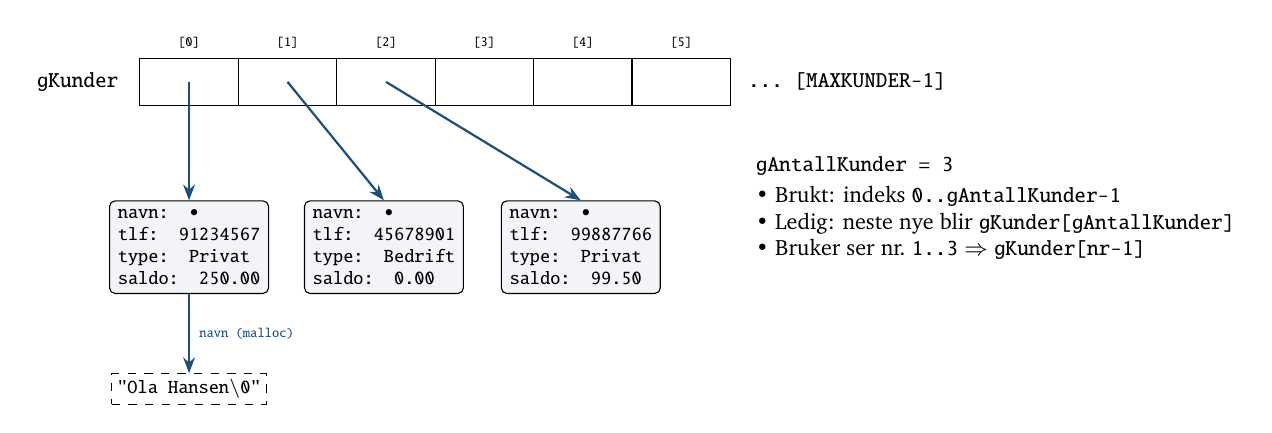
\begin{tikzpicture}[
  cell/.style={draw,minimum width=1.25cm,minimum height=0.6cm,font=\ttfamily\footnotesize},
  st/.style={draw,rounded corners=2pt,fill=frodeblue!6,font=\ttfamily\scriptsize,align=left,inner sep=3pt},
  arr/.style={-{Stealth[length=2mm]},thick,frodeblue}]
  \node[font=\ttfamily\footnotesize,anchor=east] at (-0.15,0) {gKunder};
  \foreach \i in {0,...,5} {
    \node[cell] (c\i) at (\i*1.25+0.625,0) {};
    \node[font=\ttfamily\tiny,above] at (c\i.north) {[\i]};
  }
  \node[font=\ttfamily\footnotesize,right] at (7.6,0) {\dots\ [MAXKUNDER-1]};
  \node[st] (k0) at (0.625,-2.1) {navn: \textbullet\\tlf:\ \ 91234567\\type: Privat\\saldo: 250.00};
  \node[st] (k1) at (3.1,-2.1) {navn: \textbullet\\tlf:\ \ 45678901\\type: Bedrift\\saldo: 0.00};
  \node[st] (k2) at (5.6,-2.1) {navn: \textbullet\\tlf:\ \ 99887766\\type: Privat\\saldo: 99.50};
  \draw[arr] (c0.center) -- (k0.north);
  \draw[arr] (c1.center) -- (k1.north);
  \draw[arr] (c2.center) -- (k2.north);
  \node[font=\ttfamily\scriptsize,draw,dashed,inner sep=2pt] (n0) at (0.625,-3.9) {"Ola Hansen\textbackslash0"};
  \draw[arr] (k0.south) -- (n0.north) node[midway,right,font=\ttfamily\tiny]{navn (malloc)};
  \node[font=\footnotesize,align=left,anchor=west] at (7.7,-1.6) {\texttt{gAntallKunder = 3}\\[2pt]
     \textbullet\ Brukt: indeks \texttt{0..gAntallKunder-1}\\
     \textbullet\ Ledig: neste nye blir \texttt{gKunder[gAntallKunder]}\\
     \textbullet\ Bruker ser nr.\ \texttt{1..3} $\Rightarrow$ \texttt{gKunder[nr-1]}};
\end{tikzpicture}
\end{center}

\subsection{Stil- og navneregler}
\begin{center}
\begin{tabular}{@{}L{4.3cm}L{11.3cm}@{}}
\toprule
\textbf{Regel} & \textbf{Eksempel / forklaring} \\
\midrule
Globale har \cc{g}-prefiks & \cc{gKunder}, \cc{gAntallKunder}, \cc{gBanker}. \\
To nivåer av funksjoner & \emph{Global} funksjon løper gjennom arrayen (\cc{skrivAlleKunder}); \emph{struct-funksjonen} jobber på \textbf{én} struct via peker (\cc{kundeSkrivData}). Frode: «hver skriver seg selv». \\
Navn på struct-funksjoner & \cc{<struct><Verb>}: \cc{kundeLesData}, \cc{kundeSkrivData}, \cc{kundeFrigi}, \cc{kundeLesFraFil}. \\
\cc{const} når den bare leser & \cc{void kundeSkrivData(const struct Kunde* kunde)} -- uten \cc{const} når den endrer. \\
Array-størrelser med \cc{\#define} & \cc{\#define MAXKUNDER 100} (brukes i array-deklarasjoner). Andre konstanter som \cc{const int}. \\
Ny-funksjoner sjekker plass & \cc{if (gAntallKunder < MAXKUNDER)} \dots\ \cc{else} «Fullt». \\
Andre funksjoner sjekker tom & \cc{if (gAntallKunder > 0)} \dots\ \cc{else} «Ingen registrert». \\
Datoer/klokkeslett som \cc{int} & \cc{MMDD} og \cc{TTMM}: \cc{mnd = dato/100}, \cc{dag = dato\%100} (se \ref{sec:dato}). \\
Kommentarer & Korte kommentarer til høyre for koden. Doxygen-blokker (\cc{/** @param */}) trengs ikke på eksamen. \\
\bottomrule
\end{tabular}
\end{center}
               % 9 Programskjelettet i Frodes stil
% !TEX root = ../frode-bibelen.tex
% ----------------------------------------------------------------------------
%  Frode-bibelen -- 10 LesData.h -- verktøykassen
%  Inkluderes fra frode-bibelen.tex (kompiler alltid hovedfilen).
% ----------------------------------------------------------------------------

% ====================================================== 10 LESDATA.H ========
\kapittel{\texorpdfstring{\cc{LesData.h}}{LesData.h} -- verktøykassen}\label{kap:lesdata}

\cc{LesData.h} (EKS\_34/35, \href{https://frh.folk.ntnu.no/grprog/eksempler/LesData.h}{\cc{grprog/eksempler/LesData.h}})
inkluderes med \lstinline|#include "LesData.h"| og brukes i \emph{alle} løsningsforslag.
Den inkluderer selv \cc{ctype.h}, \cc{stdio.h}, \cc{stdlib.h} og \cc{string.h}.

\begin{center}
\begin{tabular}{@{}L{6.4cm}L{9.2cm}@{}}
\toprule
\textbf{Funksjon} & \textbf{Hva den gjør -- og typisk bruk} \\
\midrule
\cc{char lesChar(const char* t)} &
Skriver \cc{t:}, leser \emph{ett} tegn og returnerer det som \textbf{stor bokstav}. \newline
\cc{kommando = lesChar("\bs nValg");} \\
\cc{int lesInt(const char* t,} \newline \cc{\ \ \ \ \ \ \ \ const int min, const int max)} &
Skriver \cc{t (min - max):} og spør \textbf{igjen og igjen} til tallet er i $[\mathit{min}, \mathit{max}]$. \newline
\cc{nr = lesInt("\bs tKundenr", 1, gAntallKunder);} \\
\cc{float lesFloat(const char* t,} \newline \cc{\ \ \ \ \ \ \ \ const float min, const float max)} &
Som \cc{lesInt}, men for desimaltall (viser grensene med 2 desimaler). \newline
\cc{k->saldo = lesFloat("\bs tSaldo", 0, 100000);} \\
\cc{char* lagOgLesText(const char* t)} &
Leser en tekst, \textbf{\cc{malloc}-er nøyaktig nok plass} og returnerer pekeren. Må \cc{free}-es senere! \newline
\cc{k->navn = lagOgLesText("\bs tNavn");} \\
\cc{void lesText(const char* t,} \newline \cc{\ \ \ \ \ \ \ \ char* tekst, const int len)} &
Leser en tekst inn i et \textbf{ferdig buffer} (maks \cc{len}-1 tegn) og fjerner \cc{'\bs n'} på slutten. \newline
\cc{char buffer[STRLEN];  lesText("\bs tNavn", buffer, STRLEN);} \\
\bottomrule
\end{tabular}
\end{center}

\begin{felle}[{Feller med LesData.h}]
\begin{itemize}
  \item \cc{lesChar} returnerer \textbf{store} bokstaver: sammenlign med \cc{'J'}, \cc{'Q'}, \cc{'R'} -- aldri \cc{'j'}.
  \item \cc{lesInt(t, 1, gAntallKunder)} når \cc{gAntallKunder == 0} gir en \textbf{evig løkke} (ingen tall er mellom 1 og 0).
        Sjekk \lstinline|if (gAntallKunder > 0)| først -- eller bruk \cc{0} som «angre» (\cc{lesInt(t, 0, gAntallKunder)}).
  \item Brukeren skriver nummer \cc{1..antall}, arrayen bruker indeks \cc{0..antall-1}: \lstinline|gKunder[nr-1]|.
  \item \cc{lagOgLesText} lager \emph{ny} memory hver gang. Lagres teksten ikke (f.eks.\ duplikat), må du \cc{free} den.
  \item Alle funksjonene leser bort avsluttende \cc{'\bs n'} (med \cc{getchar()}), så de kan blandes fritt.
        Bruker du \cc{scanf} selv, må du også gjøre \lstinline|getchar();| før neste \cc{fgets}.
\end{itemize}
\end{felle}

\begin{tips}[{Ledetekster i Frodes stil}]
Ledetekster starter ofte med \cc{"\bs t"} for innrykk, og \cc{0} brukes som «ingen/angre»:\par
\lstinline|int nr = lesInt("\tFjern kunde (0 = angre)", 0, gAntallKunder);|
\end{tips}

\subsection{Kildekoden (din egen utskrift)}
\IfFileExists{LesData.h}{%
  \lstinputlisting[inputencoding=latin1,basicstyle=\ttfamily\scriptsize]{LesData.h}%
}{%
\begin{regel}[{Legg inn originalen her}]
Last ned \href{https://frh.folk.ntnu.no/grprog/eksempler/LesData.h}{\cc{LesData.h}} fra emnesiden,
legg filen i samme mappe som \cc{frode-bibelen.tex} og kompiler på nytt -- da settes hele kildekoden inn her automatisk.
(Alternativt: skriv den ut separat og legg den bak dette arket.)
\end{regel}
}
                % 10 LesData.h -- verktøykassen
% !TEX root = ../frode-bibelen.tex
% ----------------------------------------------------------------------------
%  Frode-bibelen -- 11 Struct, pekere og memory
%  Inkluderes fra frode-bibelen.tex (kompiler alltid hovedfilen).
% ----------------------------------------------------------------------------

% ================================================== 11 STRUCT/PEKERE ========
\kapittel{Struct, pekere og memory}

\subsection{Pekere på én side}
\begin{center}
\begin{tabular}{@{}L{3.6cm}L{12.0cm}@{}}
\toprule
\cc{int* p;} & Lager en peker som kan peke på en \cc{int}. \\
\cc{p = \&x;} & \cc{\&x} = adressen til \cc{x}. Nå peker \cc{p} på \cc{x}. \\
\cc{*p = 7;} & \cc{*p} = verdien der \cc{p} peker (her: setter \cc{x} til 7). \\
\cc{t == \&t[0]} & Navnet på en array \textbf{er} adressen til første element. \\
\cc{*(t+i) == t[i]} & Pekeraritmetikk: \cc{t+i} peker \cc{i} plasser lenger ut. \\
\cc{p->navn} & Medlem via peker til struct. Samme som \cc{(*p).navn}. \\
\cc{s.navn} & Medlem i en struct-\emph{variabel} (ikke peker). \\
\cc{NULL} & «Peker ikke på noe». \cc{if (p)} = \cc{if (p != NULL)}. \\
\bottomrule
\end{tabular}
\end{center}

\subsection{\texorpdfstring{\cc{malloc}}{malloc} og \texorpdfstring{\cc{free}}{free}}
\begin{kode}
struct Kunde* ny = (struct Kunde*) malloc(sizeof(struct Kunde));   //  Én struct.
char* t  = (char*) malloc((strlen(buffer) + 1) * sizeof(char));    //  Én tekst.
int*  a  = (int*)  malloc(n * sizeof(int));                        //  Array med n int.

free(kunde->navn);       //  1) Først det som er malloc-et INNI structen,
free(kunde);             //  2) så selve structen.   (Omvendt rekkefølge = minnelekkasje.)
\end{kode}

\subsection{Array \emph{av} structer vs.\ array \emph{med pekere til} structer}
Begge varianter har vært på eksamen (S26 hadde begge i samme program).
\begin{center}
\begin{tabular}{@{}L{3.0cm}L{6.1cm}L{6.5cm}@{}}
\toprule
 & \textbf{Array av structer} & \textbf{Array med pekere (vanligst)} \\
\midrule
Deklarasjon & \cc{struct Glass gGlass[MAXGLASS];} & \cc{struct Kunde* gKunder[MAXKUNDER];} \\
Tilgang & \cc{gGlass[i].bredde} & \cc{gKunder[i]->navn} \\
Sende til funksjon & \cc{glassSkriv(gGlass[i])} (kopi) eller \newline \cc{glassLes(\&gGlass[i])} (original) & \cc{kundeSkrivData(gKunder[i])} \newline (er allerede en peker) \\
Opprette ny & ingenting -- plassen finnes & \cc{gKunder[n] = (struct Kunde*)} \newline \cc{\ \ malloc(sizeof(struct Kunde));} \\
Slette & ikke aktuelt / flytt innhold & \cc{free} inni, \cc{free} structen, flytt siste peker inn \\
\bottomrule
\end{tabular}
\end{center}

\subsection{Typiske ting \emph{inni} en struct}
\begin{kode}
struct Fugl {
  char* navn;                   //  Dynamisk tekst.
  int   antObs;                 //  Teller  +  array som brukes 0..antObs-1
  int   observasjoner[365];     //    (som gKunder/gAntallKunder, men inni structen).
  bool  dag[31];                //  Ja/nei for hver dag  ->  dag[d-1] for dag nr. d
  int   bankNr[2];              //  INDEKSER inn i en annen global array (relasjon):
};                              //    gBanker[ kunde->bankNr[0] ]->navn

struct Kunde {
  int   glass[MAXGLASS];        //  Antall bestilt av glass nr. i (S26): én teller
};                              //    per element i en annen global array.
\end{kode}

\begin{tips}[{Kopi av struct er «grunn»}]
\lstinline|*s1 = *s2;| kopierer alle medlemmene -- men for en \cc{char*} kopieres bare \emph{pekeren}.
Begge structene peker da på samme tekst. (\cc{char navn[30]} inni structen blir derimot kopiert.)
\end{tips}

\subsection{Datoer og klokkeslett som heltall}\label{sec:dato}
Frode lagrer ofte dato som \cc{MMDD} (H22, H23, S26) og klokkeslett som \cc{TTMM} (H22):
\begin{kode}
int dato = 1224;                        //  24. desember
int mnd  = dato / 100;                  //  12
int dag  = dato % 100;                  //  24
printf("%02i/%02i", dag, mnd);          //  24/12

int dato2 = mnd * 100 + dag;            //  Tilbake til MMDD.
if (dato1 < dato2)  ...                 //  MMDD kan sammenlignes direkte (samme år).

int klokken = 1430;                     //  14:30
int minutterEtterMidnatt = (klokken / 100) * 60 + klokken % 100;   //  870

const int DAGERIMND[12] = { 31,28,31,30,31,30,31,31,30,31,30,31 };
int dagNr = dag;                                    //  Dag nummer i året (1..365):
for (int m = 0;  m < mnd-1;  m++)  dagNr += DAGERIMND[m];
\end{kode}
          % 11 Struct, pekere og memory
% !TEX root = ../frode-bibelen.tex
% ----------------------------------------------------------------------------
%  Frode-bibelen -- 12 Maler: standardoperasjoner i oppgave 2
%  Inkluderes fra frode-bibelen.tex (kompiler alltid hovedfilen).
% ----------------------------------------------------------------------------

% ========================================================== 12 MALER ========
\kapittel{Maler: standardoperasjoner i oppgave 2}

Alle malene bruker skjelettet fra kapittel~\ref{kap:skjelett} (\cc{gKunder}, \cc{gAntallKunder}, \cc{struct Kunde}).
Bytt navn, behold strukturen. Frode unngår \emph{æøå} i \cc{printf}-tekster (konsollen viser dem ofte feil): skriv \cc{aa}, \cc{o}, \cc{ae}.

\subsection{Skriv alle}\label{sec:skrivalle}
\begin{kode}
void skrivAlleKunder()  {
  if (gAntallKunder > 0)  {                        //  Kunder finnes:
     printf("\n\tAlle kundene:\n");
     for (int i = 0;  i < gAntallKunder;  i++)  {
         printf("\t%3i:  ", i+1);                   //  Nummer for brukeren.
         kundeSkrivData(gKunder[i]);                //  Hver skriver seg selv.
     }
  } else
     printf("\n\tIngen kunder registrert enda!\n");
}

void kundeSkrivData(const struct Kunde* kunde)  {
  printf("%-25s  tlf: %8i  %-7s  saldo: %9.2f\n", kunde->navn, kunde->tlf,
         (kunde->type == Privat) ? "Privat" : "Bedrift", kunde->saldo);
}
\end{kode}

\subsection{Ny}\label{sec:ny}
\begin{kode}
void nyKunde()  {
  if (gAntallKunder < MAXKUNDER)  {                //  Plass til flere:
     gKunder[gAntallKunder] = (struct Kunde*) malloc(sizeof(struct Kunde));
     kundeLesData(gKunder[gAntallKunder]);         //  Leser selv sine data.
     gAntallKunder++;                              //  Én flere.
     printf("\n\tNy kunde registrert som nr.%i\n", gAntallKunder);
  } else                                           //  Fullt:
     printf("\n\tFullt med %i kunder allerede!\n", MAXKUNDER);
}
\end{kode}

\subsection{Les data inn i én struct}\label{sec:lesdata}
\begin{kode}[escapeinside={(*@}{@*)}]
void kundeLesData(struct Kunde* kunde)  {
  kunde->navn  = lagOgLesText("\tNavn");                  //  Tekst (malloc).
  kunde->tlf   = lesInt("\tTelefon", 10000000, 99999999); //  Heltall.
  kunde->type  = lesType();                               //  enum - se (*@{\ttfamily\footnotesize\color{cm}\ref{sec:enum}}@*).
  kunde->saldo = lesFloat("\tSaldo", 0, 1000000);         //  Desimaltall.

  //  Har structen en array og/eller teller? NULLSTILL dem (malloc gir søppel):
  //  kunde->antBest = 0;
  //  for (int i = 0;  i < MAXGLASS;  i++)  kunde->glass[i] = 0;
}
\end{kode}

\subsection{Ny med unikt navn (sjekk duplikat først)}\label{sec:unik}
\begin{kode}
int finnKunde(const char* navn)  {                 //  Indeks eller -1.
  for (int i = 0;  i < gAntallKunder;  i++)
      if (!strcmp(gKunder[i]->navn, navn))  return i;
  return -1;
}

void nyKunde2()  {
  char* navn;
  if (gAntallKunder < MAXKUNDER)  {
     navn = lagOgLesText("\tNavn");
     if (finnKunde(navn) == -1)  {                 //  Navnet er ledig:
        gKunder[gAntallKunder] = (struct Kunde*) malloc(sizeof(struct Kunde));
        gKunder[gAntallKunder]->navn = navn;       //  Bruker allerede lest navn,
        kundeLesResten(gKunder[gAntallKunder]);    //    leser resten (uten navn).
        gAntallKunder++;
     } else  {                                     //  Navnet finnes:
        printf("\n\tFinnes allerede en kunde med dette navnet!\n");
        free(navn);                                //  Skal IKKE lagres - frigi!
     }
  } else
     printf("\n\tFullt med %i kunder allerede!\n", MAXKUNDER);
}
\end{kode}

\subsection{Velg én og skriv alt om den}\label{sec:velgen}
\begin{kode}
void skrivEnKunde()  {                             //  Valg via NUMMER:
  if (gAntallKunder > 0)  {
     int nr = lesInt("\tKundenr", 1, gAntallKunder);
     kundeSkrivAlt(gKunder[nr-1]);                 //  nr-1 = indeks!
  } else
     printf("\n\tIngen kunder registrert enda!\n");
}

void skrivEnKundeNavn()  {                         //  Valg via NAVN:
  char buffer[STRLEN];
  int  indeks;
  lesText("\tNavn", buffer, STRLEN);
  indeks = finnKunde(buffer);
  if (indeks != -1)  kundeSkrivAlt(gKunder[indeks]);
  else  printf("\n\tIngen kunde med navnet '%s'!\n", buffer);
}
\end{kode}

\subsection{Endre / registrere noe på én}\label{sec:endre}
\begin{kode}
void endreSaldo()  {
  int nr;
  if (gAntallKunder > 0)  {
     nr = lesInt("\tEndre saldo for kundenr (0 = angre)", 0, gAntallKunder);
     if (nr != 0)  kundeEndreSaldo(gKunder[nr-1]);
     else          printf("\n\tOK - ingen endring.\n");
  } else
     printf("\n\tIngen kunder registrert enda!\n");
}

void kundeEndreSaldo(struct Kunde* kunde)  {
  printf("\n\tNaavaerende saldo: %.2f\n", kunde->saldo);
  kunde->saldo = lesFloat("\tNy saldo", 0, 1000000);
}

void kundeEndreNavn(struct Kunde* kunde)  {        //  Bytte ut en dynamisk tekst:
  free(kunde->navn);                               //    frigi gammel FØRST,
  kunde->navn = lagOgLesText("\tNytt navn");       //    lag og les ny.
}

void kundeNyBestilling(struct Kunde* kunde)  {     //  Legge til i array INNI struct:
  if (kunde->antBest < MAXBEST)
     kunde->best[kunde->antBest++] = lesInt("\tVarenr", 1, 999);
  else
     printf("\n\tFullt med bestillinger for denne kunden!\n");
}
\end{kode}

\subsection{Fjern / slett én}\label{sec:slett}
\begin{kode}
void fjernKunde()  {
  int nr;
  if (gAntallKunder > 0)  {
     nr = lesInt("\tFjern kundenr (0 = angre)", 0, gAntallKunder);
     if (nr != 0)  {
        kundeFrigi(gKunder[nr-1]);                 //  1) Frigi memory INNI structen.
        free(gKunder[nr-1]);                       //  2) Frigi selve structen.
        gKunder[nr-1] = gKunder[gAntallKunder-1];  //  3) Flytt SISTE inn i hullet.
        gKunder[gAntallKunder-1] = NULL;           //     (ryddig, ikke påkrevd)
        gAntallKunder--;                           //  4) Én færre.
        printf("\n\tKunden er fjernet.\n");
     } else
        printf("\n\tOK - ingen kunde ble fjernet.\n");
  } else
     printf("\n\tIngen kunder registrert enda!\n");
}

void kundeFrigi(struct Kunde* kunde)  {
  free(kunde->navn);                               //  ALLE char* som er malloc-et.
}
//  Frodes kompakte variant av 3) og 4):   gKunder[nr-1] = gKunder[--gAntallKunder];

//  Må REKKEFØLGEN bevares? Skyv alle bak hullet ett hakk fram i stedet for 3):
for (int i = nr-1;  i < gAntallKunder-1;  i++)  gKunder[i] = gKunder[i+1];
gAntallKunder--;
\end{kode}

\subsection{Skriv alle som matcher}\label{sec:match}
\begin{kode}
void skrivAlleAvType()  {
  enum Type type;
  bool funn = false;                               //  Foreløpig ingen funn.
  if (gAntallKunder > 0)  {
     type = lesType();
     for (int i = 0;  i < gAntallKunder;  i++)
         if (kundeErType(gKunder[i], type))  {     //  Match:
            funn = true;
            printf("\t%3i:  ", i+1);
            kundeSkrivData(gKunder[i]);
         }
     if (!funn)  printf("\n\tIngen kunder av denne typen!\n");
  } else
     printf("\n\tIngen kunder registrert enda!\n");
}

bool kundeErType(const struct Kunde* kunde, const enum Type type)  {
  return (kunde->type == type);
}

//  Søk på DEL av navn i stedet:
char sok[STRLEN];
lesText("\tSok etter (del av) navn", sok, STRLEN);
... if (strstr(gKunder[i]->navn, sok))  { ... }
\end{kode}

\subsection{Statistikk: sum, snitt, størst, flest}\label{sec:statistikk}
\begin{kode}
//  a) Sum og gjennomsnitt  (pass på heltallsdivisjon og deling på 0):
float sum = 0;
for (int i = 0;  i < gAntallKunder;  i++)  sum += gKunder[i]->saldo;
if (gAntallKunder > 0)  printf("\tSnitt: %.2f\n", sum / gAntallKunder);
//    int-summer:  (float) sumInt / antall          prosent:  100.0 * del / total

//  b) Største (husk INDEKSEN, ikke bare verdien):
int maksInd = 0;
for (int i = 1;  i < gAntallKunder;  i++)
    if (gKunder[i]->saldo > gKunder[maksInd]->saldo)  maksInd = i;
kundeSkrivData(gKunder[maksInd]);

//  c) Tell opp i en hjelpearray, finn så den største (H23, H24, H25, S25):
void dagMedFlest()  {
  int antall[ANTDAG] = { 0 };            //  ANTDAG må være #define for = { 0 }.
  int storst = -1, dagen = -1;
  for (int i = 0;  i < gAntallDeltagere;  i++)     //  For hver deltager,
      for (int d = 0;  d < ANTDAG;  d++)           //    og hver dag:
          if (gDeltagere[i]->dag[d])  antall[d]++; //  Tell opp.
  for (int d = 0;  d < ANTDAG;  d++)               //  Finn største:
      if (antall[d] > storst)  {  storst = antall[d];  dagen = d;  }
  printf("\tDag %i har flest: %i stk\n", dagen+1, storst);

  printf("\tAlle dager med %i stk:", storst);      //  Kan være FLERE like store:
  for (int d = 0;  d < ANTDAG;  d++)
      if (antall[d] == storst)  printf("  %i", d+1);
  printf("\n");
}

//  d) Tell per enum-verdi - enum-verdien ER indeksen:
int antPerType[2] = { 0 };
for (int i = 0;  i < gAntallKunder;  i++)  antPerType[gKunder[i]->type]++;
\end{kode}

\begin{tips}[{La struct-funksjonen gjøre tellejobben}]
Frode sender ofte telle-arrayen inn til struct-funksjonen, som legger til «sine» tall:\par
\lstinline|void fuglTellObservasjoner(const struct Fugl* fugl, int antall[]);|\par
Arrayen er original (ikke kopi), så økningene blir med tilbake til kalleren.
\end{tips}

\subsection{\texorpdfstring{\cc{enum}}{enum}: lese, skrive, konvertere}\label{sec:enum}
\begin{kode}
enum Type lesType()  {                       //  To verdier: ternær operator.
  char tegn;
  do  {
    tegn = lesChar("\tType (P = Privat, B = Bedrift)");
  } while (tegn != 'P'  &&  tegn != 'B');    //  Godtar KUN lovlige bokstaver.
  return (tegn == 'P') ? Privat : Bedrift;
}

enum Kategori tilKategori(const char tegn)  {   //  Mange verdier: switch.
  switch (tegn)  {
    case 'H':  return Hentes;
    case 'L':  return Lagres;
    case 'S':  return Selges;
    default:   return Ubestemt;
  }
}

void skrivType(const enum Type type)  {      //  enum -> tekst med switch,
  switch (type)  {
    case Privat:   printf("Privat ");   break;
    case Bedrift:  printf("Bedrift");   break;
  }
}
const char* gTypeTekst[] = { "Privat", "Bedrift" };   //  ... eller med tekst-array
printf("%s", gTypeTekst[kunde->type]);                //  (samme rekkefølge som enum).
\end{kode}

\subsection{Sortering (boblesortering av pekerne)}\label{sec:sortering}
\begin{kode}
void sorterKunderPaaNavn()  {
  struct Kunde* hjelp;
  for (int i = 0;  i < gAntallKunder-1;  i++)
      for (int j = 0;  j < gAntallKunder-1-i;  j++)
          if (strcmp(gKunder[j]->navn, gKunder[j+1]->navn) > 0)  {  //  Feil rekkefølge:
             hjelp = gKunder[j];   gKunder[j] = gKunder[j+1];   gKunder[j+1] = hjelp;
          }
}
//  Tall, synkende:   if (gKunder[j]->saldo < gKunder[j+1]->saldo)  { ...bytt... }
\end{kode}

\subsection{Slett alt ved programslutt}
\begin{kode}
void slettAlleKunder()  {
  for (int i = 0;  i < gAntallKunder;  i++)  {
      kundeFrigi(gKunder[i]);   free(gKunder[i]);
  }
  gAntallKunder = 0;
}
\end{kode}
                  % 12 Maler: standardoperasjoner i oppgave 2
% !TEX root = ../frode-bibelen.tex
% ----------------------------------------------------------------------------
%  Frode-bibelen -- 13 Filer
%  Inkluderes fra frode-bibelen.tex (kompiler alltid hovedfilen).
% ----------------------------------------------------------------------------

% ========================================================== 13 FILER ========
\kapittel{Filer}

\begin{regel}[{Gullregel: filformat}]
Les \textbf{nøyaktig} det formatet oppgaven beskriver -- og skriv \textbf{nøyaktig} det samme når du skriver til fil.
\cc{xxxLesFraFil} og \cc{xxxSkrivTilFil} skal være speilbilder av hverandre.
\end{regel}

\begin{center}
\begin{tabular}{@{}L{5.6cm}L{10.0cm}@{}}
\toprule
\textbf{På fila står \dots} & \textbf{Les med \dots} \\
\midrule
ett tall & \cc{fscanf(inn, "\%i", \&x);} \\
flere tall/tegn på samme linje & \cc{fscanf(inn, "\%i \%c \%f", \&(k->tlf), \&tegn, \&(k->saldo));} \\
blank før tekst / \cc{'\bs n'} etter tall & \cc{getc(inn);} \ (leser og forkaster \emph{ett} tegn) \\
tekst ut linja (kan ha blanke) & \cc{fgets(buffer, STRLEN, inn);} \cc{buffer[strlen(buffer)-1] = '\bs 0';} \\
ett ord (ingen blanke) & \cc{fscanf(inn, "\%s", buffer);} \\
\cc{0}/\cc{1} som skal bli \cc{bool} & \cc{fscanf(inn, "\%i", \&kan);} \cc{k->dag[i] = (kan == 1);} \\
bokstav som skal bli \cc{enum} & \cc{fscanf(inn, " \%c", \&tegn);} \cc{k->type = (tegn == 'P') ? Privat : Bedrift;} \\
antall + så mange verdier & \cc{fscanf} antallet, deretter en \cc{for}-løkke med \cc{fscanf}, til slutt \cc{getc}. \\
\bottomrule
\end{tabular}
\end{center}

\subsection{Les fra fil -- antallet står først}\label{sec:lesfil}
Filformat (eksempel):
\begin{kode}[language={},backgroundcolor=\color{white}]
3
91234567 P 250.00 Ola Hansen
45678901 B 0.00 Fjellsport AS
99887766 P 99.50 Kari Nordmann
\end{kode}
\begin{kode}
void lesFraFil()  {
  FILE* innfil = fopen("KUNDER.DTA", "r");             //  Åpner for lesing.
  if (innfil)  {                                       //  Filen finnes:
     fscanf(innfil, "%i", &gAntallKunder);             //  Leser antallet,
     getc(innfil);                                     //    og '\n' etter det.
     for (int i = 0;  i < gAntallKunder;  i++)  {      //  Lager og leser alle:
         gKunder[i] = (struct Kunde*) malloc(sizeof(struct Kunde));
         kundeLesFraFil(innfil, gKunder[i]);           //  Leser selv.
     }
     fclose(innfil);                                   //  Lukker INNI if-en.
     printf("\n\tKundene er lest inn fra 'KUNDER.DTA'.\n");
  } else
     printf("\n\tFant ikke filen 'KUNDER.DTA'!\n");
}

void kundeLesFraFil(FILE* inn, struct Kunde* kunde)  {
  char buffer[STRLEN];
  char tegn;
  fscanf(inn, "%i %c %f", &(kunde->tlf), &tegn, &(kunde->saldo));
  getc(inn);                                           //  Forkaster ' ' før navnet.
  fgets(buffer, STRLEN, inn);                          //  Resten av linja = navn.
  buffer[strlen(buffer)-1] = '\0';                     //  Fjerner '\n'.
  kunde->navn = (char*) malloc((strlen(buffer)+1) * sizeof(char));
  strcpy(kunde->navn, buffer);
  kunde->type = (tegn == 'P') ? Privat : Bedrift;      //  Bokstav -> enum.
}
\end{kode}

\subsection{Les fra fil -- ukjent antall (les til slutten)}
Filformat: navn på én linje, resten på neste. Les \textbf{første post før løkka} og \textbf{neste post sist i løkka} (H23).
\begin{kode}
void lesFraFil2()  {
  char buffer[STRLEN];
  FILE* innfil = fopen("KUNDER.DTA", "r");
  if (innfil)  {
     gAntallKunder = 0;
     fgets(buffer, STRLEN, innfil);                    //  Prøver å lese 1. navn.
     while (!feof(innfil)  &&  gAntallKunder < MAXKUNDER)  {
       buffer[strlen(buffer)-1] = '\0';
       gKunder[gAntallKunder] = (struct Kunde*) malloc(sizeof(struct Kunde));
       kundeLesFraFil2(innfil, gKunder[gAntallKunder], buffer);
       gAntallKunder++;
       fgets(buffer, STRLEN, innfil);                  //  Prøver å lese neste navn.
     }
     fclose(innfil);
  } else
     printf("\n\tFant ikke filen 'KUNDER.DTA'!\n");
}

void kundeLesFraFil2(FILE* inn, struct Kunde* kunde, const char* navn)  {
  char tegn;
  kunde->navn = (char*) malloc((strlen(navn)+1) * sizeof(char));
  strcpy(kunde->navn, navn);
  fscanf(inn, "%i %c %f", &(kunde->tlf), &tegn, &(kunde->saldo));
  getc(inn);                                           //  Forkaster '\n'.
  kunde->type = (tegn == 'P') ? Privat : Bedrift;
}
\end{kode}

\subsection{Skriv til fil}\label{sec:skrivfil}
\begin{kode}
void skrivTilFil()  {
  FILE* utfil = fopen("KUNDER.DTA", "w");              //  "w" OVERSKRIVER filen!
  if (utfil)  {
     fprintf(utfil, "%i\n", gAntallKunder);            //  Antallet først,
     for (int i = 0;  i < gAntallKunder;  i++)         //    så hver kunde:
         kundeSkrivTilFil(utfil, gKunder[i]);
     fclose(utfil);
  } else
     printf("\n\tKlarte ikke aa aapne 'KUNDER.DTA'!\n");
}

void kundeSkrivTilFil(FILE* ut, const struct Kunde* kunde)  {
  fprintf(ut, "%i %c %.2f %s\n", kunde->tlf,           //  SAMME format som lesingen.
          (kunde->type == Privat) ? 'P' : 'B', kunde->saldo, kunde->navn);
}
\end{kode}

\begin{center}
\begin{tabular}{@{}L{4.6cm}L{11.0cm}@{}}
\toprule
\textbf{Funksjon} & \textbf{Merk} \\
\midrule
\cc{fopen(navn, "r" | "w" | "a")} & Les / skriv (tømmer filen først) / legg til på slutten. \cc{NULL} hvis det ikke gikk. \\
\cc{fclose(fil)} & Alltid når du er ferdig -- men bare hvis \cc{fopen} lyktes. \\
\cc{fprintf(fil, format, ...)} & Som \cc{printf}, men til fil. \\
\cc{fscanf(fil, format, ...)} & Som \cc{scanf}. Hopper over blanke og \cc{'\bs n'} \emph{før} tall og \cc{\%s}. \\
\cc{fgets(buf, len, fil)} & Leser til og med \cc{'\bs n'} (eller \cc{len}-1 tegn). \textbf{Beholder} \cc{'\bs n'}. \\
\cc{getc(fil)} & Leser ett tegn (brukes for å «spise» blank eller \cc{'\bs n'}). \\
\cc{feof(fil)} & Sann først \textbf{etter} et lesforsøk som traff slutten. \\
\bottomrule
\end{tabular}
\end{center}

\begin{felle}[{Fil-feller}]
\begin{itemize}
  \item \cc{fscanf} et tall og så \cc{fgets}, \textbf{uten \cc{getc}} imellom: \cc{fgets} leser bare den tomme resten av linja (\cc{"\bs n"}).
  \item Glemt å fjerne \cc{'\bs n'} etter \cc{fgets} -- da skrives navnet med linjeskift og \cc{strcmp} finner ingenting.
  \item \cc{while (!feof(fil))} \emph{uten} å lese før løkka -- siste post leses dobbelt.
  \item \cc{fclose} utenfor \cc{if (fil)} -- \cc{fclose(NULL)} kan krasje.
  \item Test skrivingen med et annet filnavn (Frode brukte f.eks.\ \cc{.DT2}) så du ikke ødelegger datafila.
  \item Bruk filnavnet \textbf{nøyaktig} slik oppgaven oppgir det.
\end{itemize}
\end{felle}
                  % 13 Filer
% !TEX root = ../frode-bibelen.tex
% ----------------------------------------------------------------------------
%  Frode-bibelen -- 14 Lenket liste
%  Inkluderes fra frode-bibelen.tex (kompiler alltid hovedfilen).
% ----------------------------------------------------------------------------

% =================================================== 14 LENKET LISTE ========
\kapittel{Lenket liste (LIFO/FIFO)}

Pensum (forelesning 22, EKS\_32/33), men \textbf{ikke brukt på noen av eksamenene H19--S26} (verken oppgave 1 eller 2). Lav prioritet -- kjenn igjen mønsteret.


\begin{kode}
struct Person {
  char* navn;
  struct Person* neste;                  //  Peker til neste i lista (NULL = slutt).
};

struct Person* liste = NULL;             //  Tom liste.
struct Person* p;

p = (struct Person*) malloc(sizeof(struct Person));   //  LIFO: hekt inn FORREST.
p->navn  = lagOgLesText("\tNavn");
p->neste = liste;
liste    = p;

p = liste;                               //  Gå gjennom hele lista:
while (p != NULL)  {  printf("%s\n", p->navn);   p = p->neste;  }

while (liste)  {                         //  Slett hele lista:
  p = liste;   liste = liste->neste;     //  Hjelpepeker 'står igjen'.
  free(p->navn);   free(p);
}
//  FIFO (kø): ha også en peker 'siste', og hekt nye inn BAKERST:
//     if (liste == NULL) liste = p;  else siste->neste = p;     p->neste = NULL;  siste = p;
\end{kode}
           % 14 Lenket liste
% !TEX root = ../frode-bibelen.tex
% ----------------------------------------------------------------------------
%  Frode-bibelen -- 15 Eksamensarkivet H19--S26
%  Inkluderes fra frode-bibelen.tex (kompiler alltid hovedfilen).
% ----------------------------------------------------------------------------

% ================================================== 15 EKSAMENSARKIV ========
\kapittel{Eksamensarkivet H19--S26}

Alle eksamenene: 4 timer, oppgave 1 = 30\,\%, oppgave 2 = 70\,\%. Oppgave 2 er \emph{alltid} et menystyrt program med
global array av pekere (eller structer) + teller, og nesten alltid \cc{lesFraFil} som siste deloppgave.
Filene ligger på \href{https://frh.folk.ntnu.no/grprog/eksamen/}{\cc{frh.folk.ntnu.no/grprog/eksamen/}} (alt finnes også i \cc{EKSAMEN.zip}).
Kolonnen \textbf{Filer} viser prefikset. For S26 heter filene: \cc{ex\_s26.pdf} (oppgavesettet), \cc{ex\_s26\_1a.c} og \cc{ex\_s26\_1b.c}
(koden til oppgave 1 -- kjør den for å få fasit), \cc{ex\_s26\_2.c} (løsning 2) og \cc{ex\_s26\_2.tpl} (skjelett).

\begin{center}
\small
\begin{longtable}{@{}L{0.9cm}L{4.0cm}L{8.6cm}L{1.8cm}@{}}
\toprule
\textbf{Eks.} & \textbf{Oppgave 2 handler om} & \textbf{Datastruktur / spesielt} & \textbf{Filer} \\
\midrule
\endhead
\textbf{S26} & Kunder som bestiller vindusglass fra ulike produsenter & Pekere \cc{gKundene[]} + array \emph{av} structer \cc{gGlassene[]}; \cc{int glass[MAXGLASS]} teller per glasstype; kvm og faktura (\cc{float}); to datafiler. & \href{https://frh.folk.ntnu.no/grprog/eksamen/ex_s26.pdf}{\cc{ex\_s26}} \\
\textbf{H25} & Personer i en sosial gruppe og dager de kan møtes & \cc{bool dag[31]} i structen; fjern deltager (flytt siste inn); dager der alle/minst halvparten kan; 0/1 fra fil til \cc{bool}. & \href{https://frh.folk.ntnu.no/grprog/eksamen/ex_h25.pdf}{\cc{ex\_h25}} \\
\textbf{S25} & Besøk på en legevakt per ukedag og time & Fast \cc{gDogn[7]} med 24 timer hver; når det er flest besøk; skriv til og les fra fil. & \href{https://frh.folk.ntnu.no/grprog/eksamen/ex_s25.pdf}{\cc{ex\_s25}} \\
\textbf{H24} & Havner og båtrutene som går innom dem & To structer (\cc{Havn}, \cc{Rute}); en rute har opptil 20 anløp; mest travle havn via telle-array; to datafiler. & \href{https://frh.folk.ntnu.no/grprog/eksamen/ex_h24.pdf}{\cc{ex\_h24}} \\
\textbf{S24} & Én klubbs kamper og egne målscorere & Referanseoverføring \cc{kampHent(kamp, \&for, \&mot)}; poengsum og «tabellinje»; toppscorer(e). & \href{https://frh.folk.ntnu.no/grprog/eksamen/ex_s24.pdf}{\cc{ex\_s24}} \\
\textbf{H23} & Fuglearter og observasjonene av dem & \cc{antObs} + \cc{observasjoner[365]} (\cc{MMDD}) i structen; \cc{finnFugl} på navn; les fil til \cc{feof}; dag med flest observasjoner. & \href{https://frh.folk.ntnu.no/grprog/eksamen/ex_h23.pdf}{\cc{ex\_h23}} \\
\textbf{S23} & Brøytere/strøere og kundene deres & To structer; registrere brøyting/strøing; lage fakturaer; hvem som tjener mest. & \href{https://frh.folk.ntnu.no/grprog/eksamen/ex_s23.pdf}{\cc{ex\_s23}} \\
\textbf{H22} & Hendelser på en biltur i Alpene & \cc{enum Type} med 6 verdier; dato \cc{MMDD} og klokkeslett \cc{TTMM}; dato med flest hendelser. & \href{https://frh.folk.ntnu.no/grprog/eksamen/ex_h22.pdf}{\cc{ex\_h22}} \\
\textbf{S22} & Ting som må handles ved oppussing & \cc{enum Enhet}; søk på tekst; kostnad (\cc{float}) per ting. & \href{https://frh.folk.ntnu.no/grprog/eksamen/ex_s22.pdf}{\cc{ex\_s22}} \\
\textbf{H21} & Kunders lån i ulike banker & To structer (\cc{Kunde}, \cc{Bank}); \cc{bankNr[2]} som indekser inn i \cc{gBanker}; renter (\cc{float}); to datafiler. & \href{https://frh.folk.ntnu.no/grprog/eksamen/ex_h21.pdf}{\cc{ex\_h21}} \\
\textbf{S21} & Rakfisk- og pultostprodukter og produsentene & \cc{enum Type}; produsentnavn i global tekst-array; \cc{strstr}-søk; skriv til fil (\cc{.DT2}). & \href{https://frh.folk.ntnu.no/grprog/eksamen/ex_s21.pdf}{\cc{ex\_s21}} \\
\textbf{H20} & Gjenstander som skal ryddes ut av et hus & \cc{enum Kategori} med 6 verdier; skriv alle i én kategori; endre kategori; skriv til og les fra fil. & \href{https://frh.folk.ntnu.no/grprog/eksamen/ex_h20.pdf}{\cc{ex\_h20}} \\
\textbf{S20} & Episoder sett i sesongene av en lang serie & Episoder per sesong i structen; søk på sesongnavn (egen \cc{bool}-funksjon); prosentvis sett. & \href{https://frh.folk.ntnu.no/grprog/eksamen/ex_s20.pdf}{\cc{ex\_s20}} \\
\textbf{H19} & Ansatte, arbeidsdager og oppmøte & Dager i måneden per ansatt; registrere oppmøte; statistikk; to datafiler (ansatte og jobbing). & \href{https://frh.folk.ntnu.no/grprog/eksamen/ex_h19.pdf}{\cc{ex\_h19}} \\
\bottomrule
\end{longtable}
\end{center}

\begin{tips}[{Slik øver du med arkivet}]
\begin{enumerate}
  \item Last ned \cc{ex\_xxx\_2.tpl} (skjelettet) og datafilene (\cc{.dta} -- gi dem filnavnet oppgaven bruker, f.eks.\ \cc{EX\_H25\_SAMLING.DTA}).
  \item Løs oppgaven på 2,5 timer med \emph{bare} papir-hjelpemidler (denne bibelen + \cc{LesData.h}).
  \item Kompiler og test. Sammenlign med \cc{ex\_xxx\_2.c} og rettemalen -- skriv det du bommet på i margen her.
\end{enumerate}
\end{tips}
          % 15 Eksamensarkivet H19--S26
% !TEX root = ../frode-bibelen.tex
% ----------------------------------------------------------------------------
%  Frode-bibelen -- 16 Sjekkliste -- oppgave 2
%  Inkluderes fra frode-bibelen.tex (kompiler alltid hovedfilen).
% ----------------------------------------------------------------------------

% =================================================== 16 SJEKKLISTE 2 ========
\kapittel{Sjekkliste -- oppgave 2}\label{kap:sjekk2}

\subsection*{For hver funksjon du skriver}
\begin{multicols}{2}\raggedright
\boks Lest hele deloppgaven -- og hva som er ferdiglaget\\
\boks Tegnet datastrukturen\\
\boks Ny: \cc{if (gAntall < MAX)} + «Fullt»-melding\\
\boks Andre: \cc{if (gAntall > 0)} før \cc{lesInt(t, 1, gAntall)}\\
\boks Bruker \cc{nr-1} som indeks\\
\boks \cc{malloc} for ny struct \emph{og} for hver \cc{char*}\\
\boks Nullstilt tellere og arrayer i ny struct\\
\boks \cc{gAntall++} etter ny / \cc{gAntall--} etter sletting\\
\boks \cc{free} inni structen \emph{før} \cc{free} av structen\\
\columnbreak
\boks Global funksjon løkker, struct-funksjon gjør jobben\\
\boks \cc{->} for pekere, \cc{.} for struct-variable\\
\boks \cc{strcmp(\dots) == 0} for like tekster\\
\boks \cc{(float)} før deling når snitt skal ha desimaler\\
\boks Fil: \cc{getc} etter \cc{fscanf} før \cc{fgets}\\
\boks Fil: fjernet \cc{'\bs n'} etter \cc{fgets}\\
\boks Fil: \cc{fclose} inni \cc{if (fil)}\\
\boks Skriv-til-fil har \emph{samme} format som les-fra-fil\\
\boks Kommentert det jeg er usikker på
\end{multicols}

\subsection*{Siste 15 minutter}
\boks Alle deloppgaver har \emph{noe} (kode eller pseudokode) \quad \boks Ingen deloppgave står blank\\
\boks Lagret/levert i Inspera
    % 16 Sjekkliste -- oppgave 2

\end{document}
